\documentclass[
  jou,
  floatsintext,
  longtable,
  nolmodern,
  notxfonts,
  notimes,
  colorlinks=true,linkcolor=blue,citecolor=blue,urlcolor=blue]{apa7}

\usepackage{amsmath}
\usepackage{amssymb}
\usepackage{setspace}


\usepackage[bidi=default]{babel}
\babelprovide[main,import]{english}


% get rid of language-specific shorthands (see #6817):
\let\LanguageShortHands\languageshorthands
\def\languageshorthands#1{}

\RequirePackage{longtable}
\RequirePackage{threeparttablex}

\usepackage{framed}


\makeatletter
\renewcommand{\paragraph}{\@startsection{paragraph}{4}{\parindent}%
	{0\baselineskip \@plus 0.2ex \@minus 0.2ex}%
	{-.5em}%
	{\normalfont\normalsize\bfseries\typesectitle}}

\renewcommand{\subparagraph}[1]{\@startsection{subparagraph}{5}{0.5em}%
	{0\baselineskip \@plus 0.2ex \@minus 0.2ex}%
	{-\z@\relax}%
	{\normalfont\normalsize\bfseries\itshape\hspace{\parindent}{#1}\textit{\addperi}}{\relax}}
\makeatother




\usepackage{longtable, booktabs, multirow, multicol, colortbl, hhline, caption, array, float, xpatch}
\usepackage{subcaption}


\renewcommand\thesubfigure{\Alph{subfigure}}
\setcounter{topnumber}{2}
\setcounter{bottomnumber}{2}
\setcounter{totalnumber}{4}
\renewcommand{\topfraction}{0.85}
\renewcommand{\bottomfraction}{0.85}
\renewcommand{\textfraction}{0.15}
\renewcommand{\floatpagefraction}{0.7}

\usepackage{tcolorbox}
\tcbuselibrary{listings,theorems, breakable, skins}
\usepackage{fontawesome5}

\definecolor{quarto-callout-color}{HTML}{909090}
\definecolor{quarto-callout-note-color}{HTML}{0758E5}
\definecolor{quarto-callout-important-color}{HTML}{CC1914}
\definecolor{quarto-callout-warning-color}{HTML}{EB9113}
\definecolor{quarto-callout-tip-color}{HTML}{00A047}
\definecolor{quarto-callout-caution-color}{HTML}{FC5300}
\definecolor{quarto-callout-color-frame}{HTML}{ACACAC}
\definecolor{quarto-callout-note-color-frame}{HTML}{4582EC}
\definecolor{quarto-callout-important-color-frame}{HTML}{D9534F}
\definecolor{quarto-callout-warning-color-frame}{HTML}{F0AD4E}
\definecolor{quarto-callout-tip-color-frame}{HTML}{02B875}
\definecolor{quarto-callout-caution-color-frame}{HTML}{FD7E14}

%\newlength\Oldarrayrulewidth
%\newlength\Oldtabcolsep


\usepackage{hyperref}
\usepackage[protrusion=true]{microtype}



\providecommand{\tightlist}{%
  \setlength{\itemsep}{0pt}\setlength{\parskip}{0pt}}
\usepackage{longtable,booktabs,array}
\usepackage{calc} % for calculating minipage widths
% Correct order of tables after \paragraph or \subparagraph
\usepackage{etoolbox}
\makeatletter
\patchcmd\longtable{\par}{\if@noskipsec\mbox{}\fi\par}{}{}
\makeatother
% Allow footnotes in longtable head/foot
\IfFileExists{footnotehyper.sty}{\usepackage{footnotehyper}}{\usepackage{footnote}}
\makesavenoteenv{longtable}

\usepackage{graphicx}
\makeatletter
\newsavebox\pandoc@box
\newcommand*\pandocbounded[1]{% scales image to fit in text height/width
  \sbox\pandoc@box{#1}%
  \Gscale@div\@tempa{\textheight}{\dimexpr\ht\pandoc@box+\dp\pandoc@box\relax}%
  \Gscale@div\@tempb{\linewidth}{\wd\pandoc@box}%
  \ifdim\@tempb\p@<\@tempa\p@\let\@tempa\@tempb\fi% select the smaller of both
  \ifdim\@tempa\p@<\p@\scalebox{\@tempa}{\usebox\pandoc@box}%
  \else\usebox{\pandoc@box}%
  \fi%
}
% Set default figure placement to htbp
\def\fps@figure{htbp}
\makeatother


% definitions for citeproc citations
\NewDocumentCommand\citeproctext{}{}
\NewDocumentCommand\citeproc{mm}{%
  \begingroup\def\citeproctext{#2}\cite{#1}\endgroup}
\makeatletter
 % allow citations to break across lines
 \let\@cite@ofmt\@firstofone
 % avoid brackets around text for \cite:
 \def\@biblabel#1{}
 \def\@cite#1#2{{#1\if@tempswa , #2\fi}}
\makeatother
\newlength{\cslhangindent}
\setlength{\cslhangindent}{1.5em}
\newlength{\csllabelwidth}
\setlength{\csllabelwidth}{3em}
\newenvironment{CSLReferences}[2] % #1 hanging-indent, #2 entry-spacing
 {\begin{list}{}{%
  \setlength{\itemindent}{0pt}
  \setlength{\leftmargin}{0pt}
  \setlength{\parsep}{0pt}
  % turn on hanging indent if param 1 is 1
  \ifodd #1
   \setlength{\leftmargin}{\cslhangindent}
   \setlength{\itemindent}{-1\cslhangindent}
  \fi
  % set entry spacing
  \setlength{\itemsep}{#2\baselineskip}}}
 {\end{list}}
\usepackage{calc}
\newcommand{\CSLBlock}[1]{\hfill\break\parbox[t]{\linewidth}{\strut\ignorespaces#1\strut}}
\newcommand{\CSLLeftMargin}[1]{\parbox[t]{\csllabelwidth}{\strut#1\strut}}
\newcommand{\CSLRightInline}[1]{\parbox[t]{\linewidth - \csllabelwidth}{\strut#1\strut}}
\newcommand{\CSLIndent}[1]{\hspace{\cslhangindent}#1}


\usepackage[nolongtablepatch]{lineno}
\setlength\linenumbersep{5pt}
\setlength\columnsep{25pt}

\linenumbers



\usepackage{newtx}

\defaultfontfeatures{Scale=MatchLowercase}
\defaultfontfeatures[\rmfamily]{Ligatures=TeX,Scale=1}





\title{Mega-analysis of the Interoceptive Accuracy Scale (IAS) Structure
and its Dispositional Correlates}


\shorttitle{IAS Mega-analysis}


\usepackage{etoolbox}









\authorsnames[{1},{1,2},{1},{1,3},{1,4},{1,4}]{Ana Neves,Magdalena
Pfaff,Robyn Scharte,Raquel Nogueira-Arjona,Giulia L. Poerio,Dominique
Makowski}







\authorsaffiliations{
{School of Psychology, University of Sussex},{Brighton and Sussex
Medical School, University of Sussex},{Sussex Addictions Research and
Intervention Centre, University of Sussex},{Sussex Centre for
Consciousness Science, University of Sussex}}




\leftheader{Neves, Pfaff, Scharte, Nogueira-Arjona, Poerio and Makowski}



\abstract{Recent reviews demonstrate that historic questionnaires
designed to assess interoceptive abilities show low convergence and
likely measure distinct constructs. Motivated by the theoretical
distinction between interoceptive accuracy versus attention, the
Interoceptive Accuracy Scale (IAS) is a recently developed, promising,
and increasingly popular measure, but its psychometric properties and
dimensional structure remain underexplored. Across two studies, we used
a mega-analytic approach combining data from 17 datasets (N
\textgreater{} 33,000) to provide the most comprehensive evaluation to
date of the IAS, including both its structure (Study 1) and
dispositional correlates (Study 2). Study 1 triangulated the IAS
structure across multiple dimensionality-exploration algorithms,
identifying a stable core of 14-items, composed of 7 correlated but
distinct pairs of items tied to specific bodily sensations (e.g.,
Hunger--Thirst, Urinate--Defecate, Cough--Sneeze). Study 2 examined
associations between the IAS and measures of mood, anxiety,
psychopathological and neurodevelopmental traits, personality, and
belief-related constructs. Results revealed a nuanced pattern of
associations, broadly reflecting positive links with adaptive affective
and personality characteristics, and negative links with maladaptive
traits. The 14-item IAS performed comparably to the original 21-item
version, but item-pairing improved interpretability and highlightd
domain-specific patterns. In particular, the Hungry-Thirsty and
Bruise-Blood-sugar pairs displayed the strongest and most consistent
associations with relevant outcomes. Taken together, these findings
provide support for the idea that self-perceived interoceptive abilities
is a differentiated construct, varying across bodily systems. }

\keywords{Interoception, interoceptive accuracy, interoceptive
sensibility, measurement, exploratory factor analysis, network analysis}

\authornote{\par{\addORCIDlink{Ana
Neves}{0009-0006-0020-7599}}\par{\addORCIDlink{Magdalena
Pfaff}{0009-0006-2386-7936}}\par{\addORCIDlink{Robyn
Scharte}{0009-0009-8474-3496}}\par{\addORCIDlink{Raquel
Nogueira-Arjona}{0000-0002-5998-701X}}\par{\addORCIDlink{Giulia L.
Poerio}{0000-0002-2343-5109}}\par{\addORCIDlink{Dominique
Makowski}{0000-0001-5375-9967}} 

\par{     \href{https://realitybending.github.io/}{
\includegraphics[width=0.6\linewidth,height=\textheight,keepaspectratio]{rebel_logo.png}}\\  Author
roles were classified using the Contributor Role Taxonomy (CRediT;
https://credit.niso.org/) as follows:  Ana Neves:   Data
curation, Formal Analysis, Investigation, Visualization, Writing --
original draft, Writing -- review \& editing; Magdalena Pfaff:   Data
curation, Writing -- original draft; Robyn Scharte:   Writing -- review
\& editing; Raquel Nogueira-Arjona:   Writing -- review \&
editing; Giulia L. Poerio:   Writing -- review \& editing; Dominique
Makowski:   Project administration, Data curation, Formal
Analysis, Investigation, Visualization, Writing -- original
draft, Writing -- review \& editing}
\par{Correspondence concerning this article should be addressed to Ana
Neves, Email: \href{mailto:A.Neves@sussex.ac.uk}{A.Neves@sussex.ac.uk}}
}

\usepackage{pbalance}
% \usepackage{float}
\makeatletter
\let\oldtpt\ThreePartTable
\let\endoldtpt\endThreePartTable
\def\ThreePartTable{\@ifnextchar[\ThreePartTable@i \ThreePartTable@ii}
\def\ThreePartTable@i[#1]{\begin{figure}[!htbp]
\onecolumn
\begin{minipage}{0.485\textwidth}
\oldtpt[#1]
}
\def\ThreePartTable@ii{\begin{figure}[!htbp]
\onecolumn
\begin{minipage}{0.48\textwidth}
\oldtpt
}
\def\endThreePartTable{
\endoldtpt
\end{minipage}
\twocolumn
\end{figure}}
\makeatother


\makeatletter
\let\endoldlt\endlongtable		
\def\endlongtable{
\hline
\endoldlt}
\makeatother

\newenvironment{twocolumntable}% environment name
{% begin code
\begin{table*}[!htbp]%
\onecolumn%
}%
{%
\twocolumn%
\end{table*}%
}% end code

\urlstyle{same}



\usepackage{fontspec}
\usepackage{multirow}
\usepackage{multicol}
\usepackage{colortbl}
\usepackage{ulem}
\usepackage{hhline}
\newlength\Oldarrayrulewidth
\newlength\Oldtabcolsep
\usepackage{longtable}
\usepackage{array}
\usepackage{hyperref}
\usepackage{float}
\usepackage{wrapfig}
\usepackage{lscape}
\makeatletter
\@ifpackageloaded{caption}{}{\usepackage{caption}}
\AtBeginDocument{%
\ifdefined\contentsname
  \renewcommand*\contentsname{Table of contents}
\else
  \newcommand\contentsname{Table of contents}
\fi
\ifdefined\listfigurename
  \renewcommand*\listfigurename{List of Figures}
\else
  \newcommand\listfigurename{List of Figures}
\fi
\ifdefined\listtablename
  \renewcommand*\listtablename{List of Tables}
\else
  \newcommand\listtablename{List of Tables}
\fi
\ifdefined\figurename
  \renewcommand*\figurename{Figure}
\else
  \newcommand\figurename{Figure}
\fi
\ifdefined\tablename
  \renewcommand*\tablename{Table}
\else
  \newcommand\tablename{Table}
\fi
}
\@ifpackageloaded{float}{}{\usepackage{float}}
\floatstyle{ruled}
\@ifundefined{c@chapter}{\newfloat{codelisting}{h}{lop}}{\newfloat{codelisting}{h}{lop}[chapter]}
\floatname{codelisting}{Listing}
\newcommand*\listoflistings{\listof{codelisting}{List of Listings}}
\makeatother
\makeatletter
\makeatother
\makeatletter
\@ifpackageloaded{caption}{}{\usepackage{caption}}
\@ifpackageloaded{subcaption}{}{\usepackage{subcaption}}
\makeatother

% From https://tex.stackexchange.com/a/645996/211326
%%% apa7 doesn't want to add appendix section titles in the toc
%%% let's make it do it
\makeatletter
\xpatchcmd{\appendix}
  {\par}
  {\addcontentsline{toc}{section}{\@currentlabelname}\par}
  {}{}
\makeatother

%% Disable longtable counter
%% https://tex.stackexchange.com/a/248395/211326

\usepackage{etoolbox}

\makeatletter
\patchcmd{\LT@caption}
  {\bgroup}
  {\bgroup\global\LTpatch@captiontrue}
  {}{}
\patchcmd{\longtable}
  {\par}
  {\par\global\LTpatch@captionfalse}
  {}{}
\apptocmd{\endlongtable}
  {\ifLTpatch@caption\else\addtocounter{table}{-1}\fi}
  {}{}
\newif\ifLTpatch@caption
\makeatother

\begin{document}

\maketitle




\setlength\LTleft{0pt}

\resetlinenumber[1]


\ifdefined\Shaded\renewenvironment{Shaded}{\begin{snugshade}\begin{singlespace}}{\end{singlespace}\end{snugshade}}\fi


\section{Introduction}\label{introduction}

Interoception refers to sensing, interpreting and integrating
information of internal bodily stimuli by the nervous system, including
organs (e.g., heart, lungs, gut) and broader physiological tissues, to
convey the body's current state
(\citeproc{ref-khalsa2018interoception}{Khalsa, Adolphs, Cameron,
Critchley, Davenport, Feinstein, Feusner, Garfinkel, Lane, Mehling, \&
others, 2018}). Despite its recognised role in emotion recognition
(\citeproc{ref-terasawa2021effects}{Terasawa et al., 2021}) and
regulation (\citeproc{ref-zamariola2019relationship}{Zamariola et al.,
2019}), decision making
(\citeproc{ref-pollatos2023interoceptive}{Pollatos et al., 2023}),
learning (\citeproc{ref-joshi2023interoception}{Joshi et al., 2023}),
body-ownership (\citeproc{ref-raimo2021body}{Raimo et al., 2021}),
physical health (\citeproc{ref-harrison2024interoception}{Harrison \&
Pink, 2024}) and psychological health
(\citeproc{ref-nord2021disrupted}{Nord et al., 2021}), and well-being
(\citeproc{ref-ferentzi2019body}{Ferentzi et al., 2019}), the field
remains hampered by concerns over its conceptualisation and measurement
(\citeproc{ref-desmedt2022measures}{Desmedt et al., 2022},
\citeproc{ref-desmedt2025discrepancies}{2025};
\citeproc{ref-murphy2024interoception}{Murphy, 2024}).

\subsection{The Interoceptive Assessment
Puzzle}\label{the-interoceptive-assessment-puzzle}

Given interoception's centrality to brain function, many measures could
be seen as ``indirectly'' assessing (whether intentionally or not)
interoceptive processes, including indices quantifying coupling between
physiological signals and cognitive or behavioural processes (e.g.,
Heart Rate Variability), or constructs theoretically dependent on
interoceptive information (e.g., alexithymia). Critically, various
\emph{direct} measures have also been developed (see
Figure~\ref{fig-measures}), spanning ``objective'' and ``subjective''
assessments (e.g., heartbeat counting/tracking tasks \emph{vs.}
questionnaires and scales), ``explicit'' and ``implicit'' paradigms
(i.e., directing \emph{vs.} covertly measuring attention to
interoceptive processes), multiple modalities (e.g., cardioception,
respiroception, gastroception), and theoretical dimensions (e.g.,
accuracy, sensitivity, awareness). The diversity of measures reflects
the absence of a ``gold-standard'' for interoception, with each having
strengths and limitations depending on the research context and
dimension assessed (\citeproc{ref-Desmedt2023accuracy}{Desmedt et al.,
2023}; \citeproc{ref-jahedi2014}{Jahedi \& Méndez, 2014}).

\begin{figure*}[!htbp]

{\caption{{Schematic Representation of The Interoceptive Assessment
Puzzle. The different modalities of interoception (e.g., cardioception)
can be assessed directly or indirectly. Direct assessments can be
subjective or objective, depending on whether they use conscious
metacognitive appraisals or performance-based indices. Objective
interoceptive tasks can be explicit (participants must consciously
attend to interoceptive signals; e.g., the heartbeat counting task) or
implicit (measurements of interoception are covert; e.g., heartbeat
evoked potentials measured during rest). Indirect assessments evaluate
constructs typically related, or dependent on, interoceptive processes
(e.g., physiological indices such as heart rate variability or effect of
cardiac phase) or abilities (e.g., self-report measures of emotion
regulation or identification abilities).}{\label{fig-measures}}}}


\includegraphics[width=1\linewidth,height=\textheight,keepaspectratio]{figures/Figure1.png}

\end{figure*}

\subsection{Self-reported
Interoception}\label{self-reported-interoception}

Although using self-report questionnaires to measure deeply embodied
functions might seem paradoxical, recent redefinitions of interoception
emphasize the importance of metacognitive elaboration of interoceptive
information, supporting the idea that some facets such as metacognitive
beliefs, can be assessed subjectively
(\citeproc{ref-khalsa2018interoception}{Khalsa, Adolphs, Cameron,
Critchley, Davenport, Feinstein, Feusner, Garfinkel, Lane, Mehling, \&
others, 2018}; \citeproc{ref-suksasilp2022towards}{Suksasilp \&
Garfinkel, 2022}). The notion that self-reported interoception reflects
a fundamentally different aspect of conscious interoceptive processing
than objective task measures is thought to be central to understanding
the reported lack of convergence between objective and subjective
measures (\citeproc{ref-desmedt2022measures}{Desmedt et al., 2022}). For
instance, questionnaires and objective measures (HCT,
\citeproc{ref-schandry1981heart}{Schandry, 1981}; Heartbeat Detection
Task (HDT), \citeproc{ref-kleckner2015methodological}{Kleckner et al.,
2015}) show weak or no correlations, even when intended to capture the
same theoretical interoceptive dimension
(\citeproc{ref-arslanova2022}{Arslanova et al., 2022};
\citeproc{ref-brand2023}{Brand et al., 2023}; e.g., task-based accuracy
vs.~self-reported accuracy, \citeproc{ref-murphy2019}{Murphy et al.,
2019}).

Perhaps more surprisingly, lack of convergence also exists amongst
objective or subjective measures purporting to measure the same
interoceptive dimension: task-based measures targeting accuracy
typically show weak or no intercorrelations
(\citeproc{ref-brand2023}{Brand et al., 2023};
\citeproc{ref-hickman2020relationship}{Hickman et al., 2020}), and
subjective accuracy scores similarly yield weaker than expected
relationships (\citeproc{ref-vig2022questionnaires}{Vig et al., 2022}).
As well as posing substantial validity concerns, these findings raise
the possibility that even within a broad measurement domain, different
measures are targeting fundamentally different facets of interoception,
undermining replicability and hindering theoretical and empirical
progress in the field.

One striking example concerns the assessment of interoceptive
sensibility - the self-reported tendency to focus on (with or without
correctly detecting) internal sensations
(\citeproc{ref-garfinkel2015knowing}{Garfinkel et al., 2015};
\citeproc{ref-khalsa2018interoception}{Khalsa, Adolphs, Cameron,
Critchley, Davenport, Feinstein, Feusner, Garfinkel, Lane, Mehling, \&
others, 2018}). A recent systematic review suggested that questionnaires
designed to assess interoceptive sensibility may in fact measure
distinct constructs, with researchers often treating them as equivalent
despite low overall convergence
(\citeproc{ref-desmedt2022measures}{Desmedt et al., 2022}). The review
included popular measures, such as the Body Perception Questionnaire
(BPQ, \citeproc{ref-porges1993body}{Porges, 1993}), the Multidimensional
Assessment of Interoceptive Awareness (MAIA,
\citeproc{ref-mehling2012}{Mehling et al., 2012}; MAIA-2,
\citeproc{ref-mehling2018multidimensional}{Mehling et al., 2018}), the
Body Awareness Questionnaire (BAQ,
\citeproc{ref-shields1989body}{Shields et al., 1989}), the Private
subscale of the Body Consciousness Questionnaire (PBCS,
\citeproc{ref-miller1981consciousness}{Miller et al., 1981}), and the
Self-Awareness Questionnaire (SAQ,
\citeproc{ref-longarzo2015self}{Longarzo et al., 2015}) which comprised
86\% of all citations. Their low-to-moderate intercorrelations suggest
they capture different aspects of interoception rather than a common
construct, emphasizing the need for conceptual clarity regarding what
each measures, how they relate to different interoception dimensions,
and their overlap with constructs such as alexithymia and body
awareness. One avenue for addressing these issues is the investigation
of newer measures not included in prior reviews.

\subsection{The Interoceptive Accuracy Scale
(IAS)}\label{the-interoceptive-accuracy-scale-ias}

Focusing on self-perceived \emph{accuracy}, the Interoceptive Accuracy
Scale (IAS, \citeproc{ref-murphy2019}{Murphy et al., 2019}) is a
recently developed measure with rapidly growing popularity. The IAS was
designed to clarify both what and how interoception is measured, by
treating interoceptive accuracy and attention as distinct dimensions,
whereas many existing models conflate them (e.g.,
\citeproc{ref-garfinkel2015knowing}{Garfinkel et al., 2015};
\citeproc{ref-khalsa2018interoception}{Khalsa, Adolphs, Cameron,
Critchley, Davenport, Feinstein, Feusner, Garfinkel, Lane, Mehling, \&
others, 2018}). Individuals may thus report attending to bodily signals
while recognising their perception of those signals is inaccurate. This
distinction positions the IAS as the only tool specifically designed to
assess subjective interoceptive accuracy, marking a conceptual advance
in interoceptive measurement.

The IAS comprises 21 Likert-scale items assessing perceived accuracy
across physiological modalities, one item per modality such as
respiration (\emph{``I can always accurately perceive when I am
breathing fast''}), heart (\emph{``I can always accurately perceive when
my heart is beating fast''}), skin (\emph{``I can always accurately
perceive when something is going to be ticklish''}), arousal or bodily
functions like coughing (\emph{``I can always accurately perceive when I
am going to cough''}) or urinating (\emph{``I can always accurately
perceive when I need to urinate''}). Its items capture specific
interoceptive behaviors and ``objective'' experiences (albeit
subjectively reported), a notable distinction from other popular
questionnaires, such as the MAIA-2, which includes broader metacognitive
items (e.g., \emph{``I trust my body sensations''}, \emph{``I can notice
an unpleasant body sensation without worrying about it''}), and
dimensions related to attention and emotion regulation (e.g.,
Not-distracting and Not-worrying subscales respectively).

The original IAS validation study suggested a two-factor structure: one
reflecting the perception of interoceptive signals (urinate, hungry,
defecate, thirsty, pain, heart, taste, breathing, temperature, muscles,
affective touch, vomit, sexual arousal), and another comprising signals
difficult to perceive through interoception alone or reflecting socially
unacceptable functions (itch, tickle, cough, burp, bruise, blood sugar,
sneeze, wind). The authors highlight the imperfect fit of this solution
(\citeproc{ref-murphy2019}{Murphy et al., 2019, p. 127}), with
subsequent studies identifying different optimal structures.
Specifically, Brand et al. (\citeproc{ref-brand2023}{2023}) reported a
1-factor solution as best fit, whereas Lin et al.
(\citeproc{ref-lin2023}{2023}) and Campos et al.
(\citeproc{ref-campos2021}{2021}) found bifactor solutions (i.e., one
general factor above lower-level factors,
\citeproc{ref-rodriguez2016evaluating}{Rodriguez et al., 2016}). Using
Exploratory Factor Analysis (EFA), and constraining the solution to two
factors, Koike and Nomura (\citeproc{ref-koike2023}{2023}) identified a
different 2-factor structure distinguishing cutaneous (e.g., itching,
tickling, affective touch, muscle sensations) from visceral sensations
(e.g., hunger, thirst, heartbeat, breathing).

Beyond factor structure, discussion has also concerned the specificity
of individual IAS items. For instance, Murphy et al.
(\citeproc{ref-murphy2019}{2019}) note that while some items measure
direct interoceptive signals (e.g., cardioception), others capture
phenomena detectable through non-interoceptive means (e.g., ``bruising''
via skin discoloration; p.~119). Lin et al.
(\citeproc{ref-lin2023}{2023}) identify several psychometric
limitations, including five locally dependent item pairs and three items
(touch, blood sugar, bruise) with high difficulty and low
discrimination, suggesting further refinement is needed. Localisation
issues also arose, with ``itch'' and ``tickle'' mapping to the same
Chinese character and thus collapsed into a single item
(\citeproc{ref-lin2023}{Lin et al., 2023}). Campos et al.
(\citeproc{ref-campos2021}{2021}) further suggested the IAS is
predominantly unidimensional, with all items except ``tickle''
reflecting a general factor.

Regarding validity, the IAS shows positive correlations with most MAIA
facets (\citeproc{ref-gaggero2021}{Gaggero et al., 2021};
\citeproc{ref-mehling2018multidimensional}{Mehling et al., 2018}),
except the Not-Distracting and Not-Worrying subscales
(\citeproc{ref-brand2023}{Brand et al., 2023}), previously linked to
non-interoceptive abilities
(\citeproc{ref-ferentzi2021examining}{Ferentzi et al., 2021}).
Comparisons with the BPQ body awareness dimension have been mixed, with
studies reporting small positive (\citeproc{ref-brand2023}{Brand et al.,
2023}; \citeproc{ref-gaggero2021}{Gaggero et al., 2021};
\citeproc{ref-koike2023}{Koike \& Nomura, 2023}), small negative
(\citeproc{ref-lin2023}{Lin et al., 2023}), quadratic positive
(\citeproc{ref-campos2021}{Campos et al., 2021}), or no correlations
(\citeproc{ref-murphy2019}{Murphy et al., 2019}). Positive correlations
have been observed for four of five FFMQ subscales
(\citeproc{ref-baer2006using}{Baer et al., 2006};
\citeproc{ref-brand2023}{Brand et al., 2023};
\citeproc{ref-koike2023}{Koike \& Nomura, 2023}), the EDI interoceptive
awareness subscale (EDI-IA, \citeproc{ref-lin2023}{Lin et al., 2023}),
and negative correlations with the Interoceptive Confusion Questionnaire
(\citeproc{ref-brand2023}{Brand et al., 2023}; ICQ,
\citeproc{ref-brewer2016alexithymia}{Brewer et al., 2016};
\citeproc{ref-murphy2019}{Murphy et al., 2019}). Finally, the IAS'
typically small correlation with the Interoceptive Attention Scale
(IATS, \citeproc{ref-gabriele2022dissociations}{Gabriele et al., 2022};
\citeproc{ref-koike2023}{Koike \& Nomura, 2023};
\citeproc{ref-lin2023}{Lin et al., 2023}) supports the distinction
between interoceptive accuracy and attention.

Despite the theoretical challenges of assessing predictive validity, the
IAS shows consistent negative associations with alexithymia
(\citeproc{ref-brand2023}{Brand et al., 2023};
\citeproc{ref-campos2021}{Campos et al., 2021};
\citeproc{ref-koike2023}{Koike \& Nomura, 2023};
\citeproc{ref-lin2023}{Lin et al., 2023};
\citeproc{ref-murphy2019}{Murphy et al., 2019}), somatic
(\citeproc{ref-brand2023}{Brand et al., 2023};
\citeproc{ref-koike2023}{Koike \& Nomura, 2023};
\citeproc{ref-lin2023}{Lin et al., 2023}) and depressive symptoms
(\citeproc{ref-brand2023}{Brand et al., 2023};
\citeproc{ref-koike2023}{Koike \& Nomura, 2023};
\citeproc{ref-lin2023}{Lin et al., 2023}), anxiety
(\citeproc{ref-brand2023}{Brand et al., 2023}), neuroticism
(\citeproc{ref-brand2023}{Brand et al., 2023}), and self-esteem
(\citeproc{ref-murphy2019}{Murphy et al., 2019}). Together, these
findings support the IAS as measuring an adaptive aspect of
interoception, though its overlap with other interoception-related
questionnaires across theoretical dimensions further highlights
limitations of strictly orthogonal interoceptive models. While the IAS
shows promise, further refinement is needed; something the present paper
seeks to address with two aims.

Given increasing interest in interoception across psychology and
neuroscience, and the growing use of the IAS, careful scrutiny of this
novel self-report measure of interoceptive accuracy is warranted.
Therefore, the current study has two aims. First (Study 1), to clarify
the structure of the IAS using a mega-analytic approach which leverages
existing data by aggregating datasets and re-analysing them at the raw
data level. This aggregated data will then be used to contrast
traditional CFA/SEM and Hierarchical Clustering Analysis (HCA) with
newer network-based approaches (Exploratory Graph Analysis, EGA). By
triangulating results across different samples and conceptually distinct
analytical frameworks, the current paper aims to provide a more nuanced
and method-independent view of IAS structure, identifying both
convergent and potentially overlooked structural features that may not
be apparent when relying on a single analytic approach. The second aim
(Study 2) is to provide an overview of construct validity and the
dispositional correlates of the IAS, clarifying its general pattern of
associations with interoception-related constructs, mood,
psychopathological and neurodevelopmental traits, and other relevant
measures, thereby situating interoceptive questionnaires within a
broader context.

\section{Study 1}\label{study-1}

Study 1 re-analyses the factor structure of the IAS using raw data
across 17 open-access datasets (\citeproc{ref-arslanova2022}{Arslanova
et al., 2022}; \citeproc{ref-brand2022}{Brand et al., 2022};
\citeproc{ref-brand2023}{Brand et al., 2023};
\citeproc{ref-campos2021}{Campos et al., 2021};
\citeproc{ref-gaggero2021}{Gaggero et al., 2021};
\citeproc{ref-lin2023}{Lin et al., 2023};
\citeproc{ref-murphy2019}{Murphy et al., 2019};
\citeproc{ref-petzke2024somatic}{Petzke et al., 2024};
\citeproc{ref-poerio2024interoceptive}{Poerio et al., 2024};
\citeproc{ref-todd2022}{Todd et al., 2022}; \citeproc{ref-von2023}{Von
Mohr et al., 2023}). Combining studies yields a more robust and
generalizable understanding of the IAS' factor structure. However, as
studies differ in sample size, demographic characteristics, language,
and procedure, we also analyse each sample individually to add nuance to
the general picture.

\subsection{Methods}\label{methods}

\subsubsection{Datasets}\label{datasets}

We searched papers citing the original IAS validation paper
(\citeproc{ref-murphy2019}{Murphy et al., 2019}), identifying 136 (as of
01/05/2024). Inclusion required open-access raw data with individual IAS
item scores; datasets shared directly by authors were also included.
Consequently, 17 datasets were used, including five from unpublished
studies (see \textbf{Table 1}), totaling 33,526 participants (Mean =
47.96 \(\pm\) 13.1, 71.3\% Female).

\begin{twocolumntable}

\global\setlength{\Oldarrayrulewidth}{\arrayrulewidth}

\global\setlength{\Oldtabcolsep}{\tabcolsep}

\setlength{\tabcolsep}{2pt}

\renewcommand*{\arraystretch}{1}



\providecommand{\ascline}[3]{\noalign{\global\arrayrulewidth #1}\arrayrulecolor[HTML]{#2}\cline{#3}}

\begin{longtable}[c]{ccccccccc}

\caption{\label{tbl-table1}Description of the samples used in Study 1
mega-analysis.}

\tabularnewline

\ascline{0.75pt}{000000}{1-9}

\multicolumn{1}{>{}c}{\advance\leftskip by 5.0pt\relax \advance\rightskip by 5.0pt\relax \textcolor[HTML]{000000}{\fontsize{6}{12}\selectfont{{\fontspec{Times New Roman} Sample}}}} & \multicolumn{1}{>{}c}{\advance\leftskip by 5.0pt\relax \advance\rightskip by 5.0pt\relax \textcolor[HTML]{000000}{\fontsize{6}{12}\selectfont{{\fontspec{Times New Roman} Reference}}}} & \multicolumn{1}{>{}c}{\advance\leftskip by 5.0pt\relax \advance\rightskip by 5.0pt\relax \textcolor[HTML]{000000}{\fontsize{6}{12}\selectfont{{\fontspec{Times New Roman} Language}}}} & \multicolumn{1}{>{}c}{\advance\leftskip by 5.0pt\relax \advance\rightskip by 5.0pt\relax \textcolor[HTML]{000000}{\fontsize{6}{12}\selectfont{{\fontspec{Times New Roman} N}}}} & \multicolumn{1}{>{}c}{\advance\leftskip by 5.0pt\relax \advance\rightskip by 5.0pt\relax \textcolor[HTML]{000000}{\fontsize{6}{12}\selectfont{{\fontspec{Times New Roman} Difference}}}} & \multicolumn{1}{>{}c}{\advance\leftskip by 5.0pt\relax \advance\rightskip by 5.0pt\relax \textcolor[HTML]{000000}{\fontsize{6}{12}\selectfont{{\fontspec{Times New Roman} Age\ (Mean\ \ ±\ SD)}}}} & \multicolumn{1}{>{}c}{\advance\leftskip by 5.0pt\relax \advance\rightskip by 5.0pt\relax \textcolor[HTML]{000000}{\fontsize{6}{12}\selectfont{{\fontspec{Times New Roman} Range}}}} & \multicolumn{1}{>{}c}{\advance\leftskip by 5.0pt\relax \advance\rightskip by 5.0pt\relax \textcolor[HTML]{000000}{\fontsize{6}{12}\selectfont{{\fontspec{Times New Roman} Female\ \%}}}} & \multicolumn{1}{>{}c}{\advance\leftskip by 5.0pt\relax \advance\rightskip by 5.0pt\relax \textcolor[HTML]{000000}{\fontsize{6}{12}\selectfont{{\fontspec{Times New Roman} Availability}}}} \\

\ascline{0.75pt}{000000}{1-9}\endfirsthead 

\ascline{0.75pt}{000000}{1-9}

\multicolumn{1}{>{}c}{\advance\leftskip by 5.0pt\relax \advance\rightskip by 5.0pt\relax \textcolor[HTML]{000000}{\fontsize{6}{12}\selectfont{{\fontspec{Times New Roman} Sample}}}} & \multicolumn{1}{>{}c}{\advance\leftskip by 5.0pt\relax \advance\rightskip by 5.0pt\relax \textcolor[HTML]{000000}{\fontsize{6}{12}\selectfont{{\fontspec{Times New Roman} Reference}}}} & \multicolumn{1}{>{}c}{\advance\leftskip by 5.0pt\relax \advance\rightskip by 5.0pt\relax \textcolor[HTML]{000000}{\fontsize{6}{12}\selectfont{{\fontspec{Times New Roman} Language}}}} & \multicolumn{1}{>{}c}{\advance\leftskip by 5.0pt\relax \advance\rightskip by 5.0pt\relax \textcolor[HTML]{000000}{\fontsize{6}{12}\selectfont{{\fontspec{Times New Roman} N}}}} & \multicolumn{1}{>{}c}{\advance\leftskip by 5.0pt\relax \advance\rightskip by 5.0pt\relax \textcolor[HTML]{000000}{\fontsize{6}{12}\selectfont{{\fontspec{Times New Roman} Difference}}}} & \multicolumn{1}{>{}c}{\advance\leftskip by 5.0pt\relax \advance\rightskip by 5.0pt\relax \textcolor[HTML]{000000}{\fontsize{6}{12}\selectfont{{\fontspec{Times New Roman} Age\ (Mean\ \ ±\ SD)}}}} & \multicolumn{1}{>{}c}{\advance\leftskip by 5.0pt\relax \advance\rightskip by 5.0pt\relax \textcolor[HTML]{000000}{\fontsize{6}{12}\selectfont{{\fontspec{Times New Roman} Range}}}} & \multicolumn{1}{>{}c}{\advance\leftskip by 5.0pt\relax \advance\rightskip by 5.0pt\relax \textcolor[HTML]{000000}{\fontsize{6}{12}\selectfont{{\fontspec{Times New Roman} Female\ \%}}}} & \multicolumn{1}{>{}c}{\advance\leftskip by 5.0pt\relax \advance\rightskip by 5.0pt\relax \textcolor[HTML]{000000}{\fontsize{6}{12}\selectfont{{\fontspec{Times New Roman} Availability}}}} \\

\ascline{0.75pt}{000000}{1-9}\endhead



\multicolumn{1}{>{}c}{\advance\leftskip by 5.0pt\relax \advance\rightskip by 5.0pt\relax \textcolor[HTML]{000000}{\fontsize{6}{12}\selectfont{{\fontspec{Times New Roman} }}}} & \multicolumn{1}{>{}c}{\advance\leftskip by 5.0pt\relax \advance\rightskip by 5.0pt\relax \textcolor[HTML]{000000}{\fontsize{6}{12}\selectfont{{\fontspec{Times New Roman} Murphy\ et\ al.,\ (2020)}}}} & \multicolumn{1}{>{}c}{\advance\leftskip by 5.0pt\relax \advance\rightskip by 5.0pt\relax \textcolor[HTML]{000000}{\fontsize{6}{12}\selectfont{{\fontspec{Times New Roman} }}}} & \multicolumn{1}{>{}c}{\advance\leftskip by 5.0pt\relax \advance\rightskip by 5.0pt\relax \textcolor[HTML]{000000}{\fontsize{6}{12}\selectfont{{\fontspec{Times New Roman} }}}} & \multicolumn{1}{>{}c}{\advance\leftskip by 5.0pt\relax \advance\rightskip by 5.0pt\relax \textcolor[HTML]{000000}{\fontsize{6}{12}\selectfont{{\fontspec{Times New Roman} }}}} & \multicolumn{1}{>{}c}{\advance\leftskip by 5.0pt\relax \advance\rightskip by 5.0pt\relax \textcolor[HTML]{000000}{\fontsize{6}{12}\selectfont{{\fontspec{Times New Roman} }}}} & \multicolumn{1}{>{}c}{\advance\leftskip by 5.0pt\relax \advance\rightskip by 5.0pt\relax \textcolor[HTML]{000000}{\fontsize{6}{12}\selectfont{{\fontspec{Times New Roman} }}}} & \multicolumn{1}{>{}c}{\advance\leftskip by 5.0pt\relax \advance\rightskip by 5.0pt\relax \textcolor[HTML]{000000}{\fontsize{6}{12}\selectfont{{\fontspec{Times New Roman} }}}} & \multicolumn{1}{>{}c}{\advance\leftskip by 5.0pt\relax \advance\rightskip by 5.0pt\relax \textcolor[HTML]{000000}{\fontsize{6}{12}\selectfont{{\fontspec{Times New Roman} osf.io/3m5nh}}}} \\





\multicolumn{1}{>{}c}{\advance\leftskip by 5.0pt\relax \advance\rightskip by 5.0pt\relax \textcolor[HTML]{000000}{\fontsize{6}{12}\selectfont{{\fontspec{Times New Roman} Sample\ 1a}}}} & \multicolumn{1}{>{}c}{\advance\leftskip by 5.0pt\relax \advance\rightskip by 5.0pt\relax \textcolor[HTML]{000000}{\fontsize{6}{12}\selectfont{{\fontspec{Times New Roman} }}}} & \multicolumn{1}{>{}c}{\advance\leftskip by 5.0pt\relax \advance\rightskip by 5.0pt\relax \textcolor[HTML]{000000}{\fontsize{6}{12}\selectfont{{\fontspec{Times New Roman} English}}}} & \multicolumn{1}{>{}c}{\advance\leftskip by 5.0pt\relax \advance\rightskip by 5.0pt\relax \textcolor[HTML]{000000}{\fontsize{6}{12}\selectfont{{\fontspec{Times New Roman} 451}}}} & \multicolumn{1}{>{}c}{\advance\leftskip by 5.0pt\relax \advance\rightskip by 5.0pt\relax \textcolor[HTML]{000000}{\fontsize{6}{12}\selectfont{{\fontspec{Times New Roman} }}}} & \multicolumn{1}{>{}c}{\advance\leftskip by 5.0pt\relax \advance\rightskip by 5.0pt\relax \textcolor[HTML]{000000}{\fontsize{6}{12}\selectfont{{\fontspec{Times New Roman} 25.8\ ±\ 8.4}}}} & \multicolumn{1}{>{}c}{\advance\leftskip by 5.0pt\relax \advance\rightskip by 5.0pt\relax \textcolor[HTML]{000000}{\fontsize{6}{12}\selectfont{{\fontspec{Times New Roman} 18-69}}}} & \multicolumn{1}{>{}c}{\advance\leftskip by 5.0pt\relax \advance\rightskip by 5.0pt\relax \textcolor[HTML]{000000}{\fontsize{6}{12}\selectfont{{\fontspec{Times New Roman} 69.4\%}}}} & \multicolumn{1}{>{}c}{\advance\leftskip by 5.0pt\relax \advance\rightskip by 5.0pt\relax \textcolor[HTML]{000000}{\fontsize{6}{12}\selectfont{{\fontspec{Times New Roman} }}}} \\





\multicolumn{1}{>{}c}{\advance\leftskip by 5.0pt\relax \advance\rightskip by 5.0pt\relax \textcolor[HTML]{000000}{\fontsize{6}{12}\selectfont{{\fontspec{Times New Roman} Sample\ 1b}}}} & \multicolumn{1}{>{}c}{\advance\leftskip by 5.0pt\relax \advance\rightskip by 5.0pt\relax \textcolor[HTML]{000000}{\fontsize{6}{12}\selectfont{{\fontspec{Times New Roman} }}}} & \multicolumn{1}{>{}c}{\advance\leftskip by 5.0pt\relax \advance\rightskip by 5.0pt\relax \textcolor[HTML]{000000}{\fontsize{6}{12}\selectfont{{\fontspec{Times New Roman} English}}}} & \multicolumn{1}{>{}c}{\advance\leftskip by 5.0pt\relax \advance\rightskip by 5.0pt\relax \textcolor[HTML]{000000}{\fontsize{6}{12}\selectfont{{\fontspec{Times New Roman} 375}}}} & \multicolumn{1}{>{}c}{\advance\leftskip by 5.0pt\relax \advance\rightskip by 5.0pt\relax \textcolor[HTML]{000000}{\fontsize{6}{12}\selectfont{{\fontspec{Times New Roman} }}}} & \multicolumn{1}{>{}c}{\advance\leftskip by 5.0pt\relax \advance\rightskip by 5.0pt\relax \textcolor[HTML]{000000}{\fontsize{6}{12}\selectfont{{\fontspec{Times New Roman} 35.3\ ±\ 16.9}}}} & \multicolumn{1}{>{}c}{\advance\leftskip by 5.0pt\relax \advance\rightskip by 5.0pt\relax \textcolor[HTML]{000000}{\fontsize{6}{12}\selectfont{{\fontspec{Times New Roman} 18-91}}}} & \multicolumn{1}{>{}c}{\advance\leftskip by 5.0pt\relax \advance\rightskip by 5.0pt\relax \textcolor[HTML]{000000}{\fontsize{6}{12}\selectfont{{\fontspec{Times New Roman} 70.1\%}}}} & \multicolumn{1}{>{}c}{\advance\leftskip by 5.0pt\relax \advance\rightskip by 5.0pt\relax \textcolor[HTML]{000000}{\fontsize{6}{12}\selectfont{{\fontspec{Times New Roman} }}}} \\





\multicolumn{1}{>{}c}{\advance\leftskip by 5.0pt\relax \advance\rightskip by 5.0pt\relax \textcolor[HTML]{000000}{\fontsize{6}{12}\selectfont{{\fontspec{Times New Roman} Sample\ 2}}}} & \multicolumn{1}{>{}c}{\advance\leftskip by 5.0pt\relax \advance\rightskip by 5.0pt\relax \textcolor[HTML]{000000}{\fontsize{6}{12}\selectfont{{\fontspec{Times New Roman} Gaggero\ et\ al.,\ (2021)}}}} & \multicolumn{1}{>{}c}{\advance\leftskip by 5.0pt\relax \advance\rightskip by 5.0pt\relax \textcolor[HTML]{000000}{\fontsize{6}{12}\selectfont{{\fontspec{Times New Roman} English\ and\ Italian}}}} & \multicolumn{1}{>{}c}{\advance\leftskip by 5.0pt\relax \advance\rightskip by 5.0pt\relax \textcolor[HTML]{000000}{\fontsize{6}{12}\selectfont{{\fontspec{Times New Roman} 814}}}} & \multicolumn{1}{>{}c}{\advance\leftskip by 5.0pt\relax \advance\rightskip by 5.0pt\relax \textcolor[HTML]{000000}{\fontsize{6}{12}\selectfont{{\fontspec{Times New Roman} }}}} & \multicolumn{1}{>{}c}{\advance\leftskip by 5.0pt\relax \advance\rightskip by 5.0pt\relax \textcolor[HTML]{000000}{\fontsize{6}{12}\selectfont{{\fontspec{Times New Roman} 24.9\ ±\ 5.3}}}} & \multicolumn{1}{>{}c}{\advance\leftskip by 5.0pt\relax \advance\rightskip by 5.0pt\relax \textcolor[HTML]{000000}{\fontsize{6}{12}\selectfont{{\fontspec{Times New Roman} 18-58}}}} & \multicolumn{1}{>{}c}{\advance\leftskip by 5.0pt\relax \advance\rightskip by 5.0pt\relax \textcolor[HTML]{000000}{\fontsize{6}{12}\selectfont{{\fontspec{Times New Roman} 60.3\%}}}} & \multicolumn{1}{>{}c}{\advance\leftskip by 5.0pt\relax \advance\rightskip by 5.0pt\relax \textcolor[HTML]{000000}{\fontsize{6}{12}\selectfont{{\fontspec{Times New Roman} osf.io/5x9sg}}}} \\





\multicolumn{1}{>{}c}{\advance\leftskip by 5.0pt\relax \advance\rightskip by 5.0pt\relax \textcolor[HTML]{000000}{\fontsize{6}{12}\selectfont{{\fontspec{Times New Roman} Sample\ 3}}}} & \multicolumn{1}{>{}c}{\advance\leftskip by 5.0pt\relax \advance\rightskip by 5.0pt\relax \textcolor[HTML]{000000}{\fontsize{6}{12}\selectfont{{\fontspec{Times New Roman} Campos\ et\ al.,\ (2022)}}}} & \multicolumn{1}{>{}c}{\advance\leftskip by 5.0pt\relax \advance\rightskip by 5.0pt\relax \textcolor[HTML]{000000}{\fontsize{6}{12}\selectfont{{\fontspec{Times New Roman} Portuguese}}}} & \multicolumn{1}{>{}c}{\advance\leftskip by 5.0pt\relax \advance\rightskip by 5.0pt\relax \textcolor[HTML]{000000}{\fontsize{6}{12}\selectfont{{\fontspec{Times New Roman} 515}}}} & \multicolumn{1}{>{}c}{\advance\leftskip by 5.0pt\relax \advance\rightskip by 5.0pt\relax \textcolor[HTML]{000000}{\fontsize{6}{12}\selectfont{{\fontspec{Times New Roman} }}}} & \multicolumn{1}{>{}c}{\advance\leftskip by 5.0pt\relax \advance\rightskip by 5.0pt\relax \textcolor[HTML]{000000}{\fontsize{6}{12}\selectfont{{\fontspec{Times New Roman} 30.7\ ±\ 10.5}}}} & \multicolumn{1}{>{}c}{\advance\leftskip by 5.0pt\relax \advance\rightskip by 5.0pt\relax \textcolor[HTML]{000000}{\fontsize{6}{12}\selectfont{{\fontspec{Times New Roman} 18-72}}}} & \multicolumn{1}{>{}c}{\advance\leftskip by 5.0pt\relax \advance\rightskip by 5.0pt\relax \textcolor[HTML]{000000}{\fontsize{6}{12}\selectfont{{\fontspec{Times New Roman} 59.6\%}}}} & \multicolumn{1}{>{}c}{\advance\leftskip by 5.0pt\relax \advance\rightskip by 5.0pt\relax \textcolor[HTML]{000000}{\fontsize{6}{12}\selectfont{{\fontspec{Times New Roman} osf.io/j6ef3}}}} \\





\multicolumn{1}{>{}c}{\advance\leftskip by 5.0pt\relax \advance\rightskip by 5.0pt\relax \textcolor[HTML]{000000}{\fontsize{6}{12}\selectfont{{\fontspec{Times New Roman} Sample\ 4}}}} & \multicolumn{1}{>{}c}{\advance\leftskip by 5.0pt\relax \advance\rightskip by 5.0pt\relax \textcolor[HTML]{000000}{\fontsize{6}{12}\selectfont{{\fontspec{Times New Roman} Todd\ et\ al.,\ (2022)}}}} & \multicolumn{1}{>{}c}{\advance\leftskip by 5.0pt\relax \advance\rightskip by 5.0pt\relax \textcolor[HTML]{000000}{\fontsize{6}{12}\selectfont{{\fontspec{Times New Roman} English}}}} & \multicolumn{1}{>{}c}{\advance\leftskip by 5.0pt\relax \advance\rightskip by 5.0pt\relax \textcolor[HTML]{000000}{\fontsize{6}{12}\selectfont{{\fontspec{Times New Roman} 802}}}} & \multicolumn{1}{>{}c}{\advance\leftskip by 5.0pt\relax \advance\rightskip by 5.0pt\relax \textcolor[HTML]{000000}{\fontsize{6}{12}\selectfont{{\fontspec{Times New Roman} }}}} & \multicolumn{1}{>{}c}{\advance\leftskip by 5.0pt\relax \advance\rightskip by 5.0pt\relax \textcolor[HTML]{000000}{\fontsize{6}{12}\selectfont{{\fontspec{Times New Roman} 48.6.6\ ±\ 14.1*}}}} & \multicolumn{1}{>{}c}{\advance\leftskip by 5.0pt\relax \advance\rightskip by 5.0pt\relax \textcolor[HTML]{000000}{\fontsize{6}{12}\selectfont{{\fontspec{Times New Roman} 18-92*}}}} & \multicolumn{1}{>{}c}{\advance\leftskip by 5.0pt\relax \advance\rightskip by 5.0pt\relax \textcolor[HTML]{000000}{\fontsize{6}{12}\selectfont{{\fontspec{Times New Roman} 50\%*}}}} & \multicolumn{1}{>{}c}{\advance\leftskip by 5.0pt\relax \advance\rightskip by 5.0pt\relax \textcolor[HTML]{000000}{\fontsize{6}{12}\selectfont{{\fontspec{Times New Roman} osf.io/ms354}}}} \\





\multicolumn{1}{>{}c}{\advance\leftskip by 5.0pt\relax \advance\rightskip by 5.0pt\relax \textcolor[HTML]{000000}{\fontsize{6}{12}\selectfont{{\fontspec{Times New Roman} Sample\ 5}}}} & \multicolumn{1}{>{}c}{\advance\leftskip by 5.0pt\relax \advance\rightskip by 5.0pt\relax \textcolor[HTML]{000000}{\fontsize{6}{12}\selectfont{{\fontspec{Times New Roman} Arslanova\ et\ al.,\ (2022)}}}} & \multicolumn{1}{>{}c}{\advance\leftskip by 5.0pt\relax \advance\rightskip by 5.0pt\relax \textcolor[HTML]{000000}{\fontsize{6}{12}\selectfont{{\fontspec{Times New Roman} English}}}} & \multicolumn{1}{>{}c}{\advance\leftskip by 5.0pt\relax \advance\rightskip by 5.0pt\relax \textcolor[HTML]{000000}{\fontsize{6}{12}\selectfont{{\fontspec{Times New Roman} 143}}}} & \multicolumn{1}{>{}c}{\advance\leftskip by 5.0pt\relax \advance\rightskip by 5.0pt\relax \textcolor[HTML]{000000}{\fontsize{6}{12}\selectfont{{\fontspec{Times New Roman} }}}} & \multicolumn{1}{>{}c}{\advance\leftskip by 5.0pt\relax \advance\rightskip by 5.0pt\relax \textcolor[HTML]{000000}{\fontsize{6}{12}\selectfont{{\fontspec{Times New Roman} 28.5\ ±\ 7.6}}}} & \multicolumn{1}{>{}c}{\advance\leftskip by 5.0pt\relax \advance\rightskip by 5.0pt\relax \textcolor[HTML]{000000}{\fontsize{6}{12}\selectfont{{\fontspec{Times New Roman} 18-73}}}} & \multicolumn{1}{>{}c}{\advance\leftskip by 5.0pt\relax \advance\rightskip by 5.0pt\relax \textcolor[HTML]{000000}{\fontsize{6}{12}\selectfont{{\fontspec{Times New Roman} 46.8\%}}}} & \multicolumn{1}{>{}c}{\advance\leftskip by 5.0pt\relax \advance\rightskip by 5.0pt\relax \textcolor[HTML]{000000}{\fontsize{6}{12}\selectfont{{\fontspec{Times New Roman} osf.io/mp3cy}}}} \\





\multicolumn{1}{>{}c}{\advance\leftskip by 5.0pt\relax \advance\rightskip by 5.0pt\relax \textcolor[HTML]{000000}{\fontsize{6}{12}\selectfont{{\fontspec{Times New Roman} Sample\ 6}}}} & \multicolumn{1}{>{}c}{\advance\leftskip by 5.0pt\relax \advance\rightskip by 5.0pt\relax \textcolor[HTML]{000000}{\fontsize{6}{12}\selectfont{{\fontspec{Times New Roman} Brand\ et\ al.,\ (2022)}}}} & \multicolumn{1}{>{}c}{\advance\leftskip by 5.0pt\relax \advance\rightskip by 5.0pt\relax \textcolor[HTML]{000000}{\fontsize{6}{12}\selectfont{{\fontspec{Times New Roman} German}}}} & \multicolumn{1}{>{}c}{\advance\leftskip by 5.0pt\relax \advance\rightskip by 5.0pt\relax \textcolor[HTML]{000000}{\fontsize{6}{12}\selectfont{{\fontspec{Times New Roman} 619}}}} & \multicolumn{1}{>{}c}{\advance\leftskip by 5.0pt\relax \advance\rightskip by 5.0pt\relax \textcolor[HTML]{000000}{\fontsize{6}{12}\selectfont{{\fontspec{Times New Roman} }}}} & \multicolumn{1}{>{}c}{\advance\leftskip by 5.0pt\relax \advance\rightskip by 5.0pt\relax \textcolor[HTML]{000000}{\fontsize{6}{12}\selectfont{{\fontspec{Times New Roman} 43.9\ ±\ 14.5}}}} & \multicolumn{1}{>{}c}{\advance\leftskip by 5.0pt\relax \advance\rightskip by 5.0pt\relax \textcolor[HTML]{000000}{\fontsize{6}{12}\selectfont{{\fontspec{Times New Roman} 18-78}}}} & \multicolumn{1}{>{}c}{\advance\leftskip by 5.0pt\relax \advance\rightskip by 5.0pt\relax \textcolor[HTML]{000000}{\fontsize{6}{12}\selectfont{{\fontspec{Times New Roman} 78.7\%}}}} & \multicolumn{1}{>{}c}{\advance\leftskip by 5.0pt\relax \advance\rightskip by 5.0pt\relax \textcolor[HTML]{000000}{\fontsize{6}{12}\selectfont{{\fontspec{Times New Roman} osf.io/xwz6g}}}} \\





\multicolumn{1}{>{}c}{\advance\leftskip by 5.0pt\relax \advance\rightskip by 5.0pt\relax \textcolor[HTML]{000000}{\fontsize{6}{12}\selectfont{{\fontspec{Times New Roman} }}}} & \multicolumn{1}{>{}c}{\advance\leftskip by 5.0pt\relax \advance\rightskip by 5.0pt\relax \textcolor[HTML]{000000}{\fontsize{6}{12}\selectfont{{\fontspec{Times New Roman} Brand\ et\ al.,\ (2023)}}}} & \multicolumn{1}{>{}c}{\advance\leftskip by 5.0pt\relax \advance\rightskip by 5.0pt\relax \textcolor[HTML]{000000}{\fontsize{6}{12}\selectfont{{\fontspec{Times New Roman} }}}} & \multicolumn{1}{>{}c}{\advance\leftskip by 5.0pt\relax \advance\rightskip by 5.0pt\relax \textcolor[HTML]{000000}{\fontsize{6}{12}\selectfont{{\fontspec{Times New Roman} }}}} & \multicolumn{1}{>{}c}{\advance\leftskip by 5.0pt\relax \advance\rightskip by 5.0pt\relax \textcolor[HTML]{000000}{\fontsize{6}{12}\selectfont{{\fontspec{Times New Roman} }}}} & \multicolumn{1}{>{}c}{\advance\leftskip by 5.0pt\relax \advance\rightskip by 5.0pt\relax \textcolor[HTML]{000000}{\fontsize{6}{12}\selectfont{{\fontspec{Times New Roman} }}}} & \multicolumn{1}{>{}c}{\advance\leftskip by 5.0pt\relax \advance\rightskip by 5.0pt\relax \textcolor[HTML]{000000}{\fontsize{6}{12}\selectfont{{\fontspec{Times New Roman} }}}} & \multicolumn{1}{>{}c}{\advance\leftskip by 5.0pt\relax \advance\rightskip by 5.0pt\relax \textcolor[HTML]{000000}{\fontsize{6}{12}\selectfont{{\fontspec{Times New Roman} }}}} & \multicolumn{1}{>{}c}{\advance\leftskip by 5.0pt\relax \advance\rightskip by 5.0pt\relax \textcolor[HTML]{000000}{\fontsize{6}{12}\selectfont{{\fontspec{Times New Roman} osf.io/3f2h6}}}} \\





\multicolumn{1}{>{}c}{\advance\leftskip by 5.0pt\relax \advance\rightskip by 5.0pt\relax \textcolor[HTML]{000000}{\fontsize{6}{12}\selectfont{{\fontspec{Times New Roman} Sample\ 7a}}}} & \multicolumn{1}{>{}c}{\advance\leftskip by 5.0pt\relax \advance\rightskip by 5.0pt\relax \textcolor[HTML]{000000}{\fontsize{6}{12}\selectfont{{\fontspec{Times New Roman} }}}} & \multicolumn{1}{>{}c}{\advance\leftskip by 5.0pt\relax \advance\rightskip by 5.0pt\relax \textcolor[HTML]{000000}{\fontsize{6}{12}\selectfont{{\fontspec{Times New Roman} German}}}} & \multicolumn{1}{>{}c}{\advance\leftskip by 5.0pt\relax \advance\rightskip by 5.0pt\relax \textcolor[HTML]{000000}{\fontsize{6}{12}\selectfont{{\fontspec{Times New Roman} 522}}}} & \multicolumn{1}{>{}c}{\advance\leftskip by 5.0pt\relax \advance\rightskip by 5.0pt\relax \textcolor[HTML]{000000}{\fontsize{6}{12}\selectfont{{\fontspec{Times New Roman} }}}} & \multicolumn{1}{>{}c}{\advance\leftskip by 5.0pt\relax \advance\rightskip by 5.0pt\relax \textcolor[HTML]{000000}{\fontsize{6}{12}\selectfont{{\fontspec{Times New Roman} 23.4\ ±\ 6.7}}}} & \multicolumn{1}{>{}c}{\advance\leftskip by 5.0pt\relax \advance\rightskip by 5.0pt\relax \textcolor[HTML]{000000}{\fontsize{6}{12}\selectfont{{\fontspec{Times New Roman} 18-79}}}} & \multicolumn{1}{>{}c}{\advance\leftskip by 5.0pt\relax \advance\rightskip by 5.0pt\relax \textcolor[HTML]{000000}{\fontsize{6}{12}\selectfont{{\fontspec{Times New Roman} 79.5\%}}}} & \multicolumn{1}{>{}c}{\advance\leftskip by 5.0pt\relax \advance\rightskip by 5.0pt\relax \textcolor[HTML]{000000}{\fontsize{6}{12}\selectfont{{\fontspec{Times New Roman} }}}} \\





\multicolumn{1}{>{}c}{\advance\leftskip by 5.0pt\relax \advance\rightskip by 5.0pt\relax \textcolor[HTML]{000000}{\fontsize{6}{12}\selectfont{{\fontspec{Times New Roman} Sample\ 7b}}}} & \multicolumn{1}{>{}c}{\advance\leftskip by 5.0pt\relax \advance\rightskip by 5.0pt\relax \textcolor[HTML]{000000}{\fontsize{6}{12}\selectfont{{\fontspec{Times New Roman} }}}} & \multicolumn{1}{>{}c}{\advance\leftskip by 5.0pt\relax \advance\rightskip by 5.0pt\relax \textcolor[HTML]{000000}{\fontsize{6}{12}\selectfont{{\fontspec{Times New Roman} German}}}} & \multicolumn{1}{>{}c}{\advance\leftskip by 5.0pt\relax \advance\rightskip by 5.0pt\relax \textcolor[HTML]{000000}{\fontsize{6}{12}\selectfont{{\fontspec{Times New Roman} 1993}}}} & \multicolumn{1}{>{}c}{\advance\leftskip by 5.0pt\relax \advance\rightskip by 5.0pt\relax \textcolor[HTML]{000000}{\fontsize{6}{12}\selectfont{{\fontspec{Times New Roman} }}}} & \multicolumn{1}{>{}c}{\advance\leftskip by 5.0pt\relax \advance\rightskip by 5.0pt\relax \textcolor[HTML]{000000}{\fontsize{6}{12}\selectfont{{\fontspec{Times New Roman} 32.0\ ±\ 12.6}}}} & \multicolumn{1}{>{}c}{\advance\leftskip by 5.0pt\relax \advance\rightskip by 5.0pt\relax \textcolor[HTML]{000000}{\fontsize{6}{12}\selectfont{{\fontspec{Times New Roman} 16-81}}}} & \multicolumn{1}{>{}c}{\advance\leftskip by 5.0pt\relax \advance\rightskip by 5.0pt\relax \textcolor[HTML]{000000}{\fontsize{6}{12}\selectfont{{\fontspec{Times New Roman} 77.7\%}}}} & \multicolumn{1}{>{}c}{\advance\leftskip by 5.0pt\relax \advance\rightskip by 5.0pt\relax \textcolor[HTML]{000000}{\fontsize{6}{12}\selectfont{{\fontspec{Times New Roman} }}}} \\





\multicolumn{1}{>{}c}{\advance\leftskip by 5.0pt\relax \advance\rightskip by 5.0pt\relax \textcolor[HTML]{000000}{\fontsize{6}{12}\selectfont{{\fontspec{Times New Roman} Sample\ 7c}}}} & \multicolumn{1}{>{}c}{\advance\leftskip by 5.0pt\relax \advance\rightskip by 5.0pt\relax \textcolor[HTML]{000000}{\fontsize{6}{12}\selectfont{{\fontspec{Times New Roman} }}}} & \multicolumn{1}{>{}c}{\advance\leftskip by 5.0pt\relax \advance\rightskip by 5.0pt\relax \textcolor[HTML]{000000}{\fontsize{6}{12}\selectfont{{\fontspec{Times New Roman} German}}}} & \multicolumn{1}{>{}c}{\advance\leftskip by 5.0pt\relax \advance\rightskip by 5.0pt\relax \textcolor[HTML]{000000}{\fontsize{6}{12}\selectfont{{\fontspec{Times New Roman} 802}}}} & \multicolumn{1}{>{}c}{\advance\leftskip by 5.0pt\relax \advance\rightskip by 5.0pt\relax \textcolor[HTML]{000000}{\fontsize{6}{12}\selectfont{{\fontspec{Times New Roman} }}}} & \multicolumn{1}{>{}c}{\advance\leftskip by 5.0pt\relax \advance\rightskip by 5.0pt\relax \textcolor[HTML]{000000}{\fontsize{6}{12}\selectfont{{\fontspec{Times New Roman} 27.3\ ±\ 9.3}}}} & \multicolumn{1}{>{}c}{\advance\leftskip by 5.0pt\relax \advance\rightskip by 5.0pt\relax \textcolor[HTML]{000000}{\fontsize{6}{12}\selectfont{{\fontspec{Times New Roman} 18-72}}}} & \multicolumn{1}{>{}c}{\advance\leftskip by 5.0pt\relax \advance\rightskip by 5.0pt\relax \textcolor[HTML]{000000}{\fontsize{6}{12}\selectfont{{\fontspec{Times New Roman} 68.9\%}}}} & \multicolumn{1}{>{}c}{\advance\leftskip by 5.0pt\relax \advance\rightskip by 5.0pt\relax \textcolor[HTML]{000000}{\fontsize{6}{12}\selectfont{{\fontspec{Times New Roman} }}}} \\





\multicolumn{1}{>{}c}{\advance\leftskip by 5.0pt\relax \advance\rightskip by 5.0pt\relax \textcolor[HTML]{000000}{\fontsize{6}{12}\selectfont{{\fontspec{Times New Roman} }}}} & \multicolumn{1}{>{}c}{\advance\leftskip by 5.0pt\relax \advance\rightskip by 5.0pt\relax \textcolor[HTML]{000000}{\fontsize{6}{12}\selectfont{{\fontspec{Times New Roman} Lin\ et\ al.,\ (2023)}}}} & \multicolumn{1}{>{}c}{\advance\leftskip by 5.0pt\relax \advance\rightskip by 5.0pt\relax \textcolor[HTML]{000000}{\fontsize{6}{12}\selectfont{{\fontspec{Times New Roman} }}}} & \multicolumn{1}{>{}c}{\advance\leftskip by 5.0pt\relax \advance\rightskip by 5.0pt\relax \textcolor[HTML]{000000}{\fontsize{6}{12}\selectfont{{\fontspec{Times New Roman} }}}} & \multicolumn{1}{>{}c}{\advance\leftskip by 5.0pt\relax \advance\rightskip by 5.0pt\relax \textcolor[HTML]{000000}{\fontsize{6}{12}\selectfont{{\fontspec{Times New Roman} }}}} & \multicolumn{1}{>{}c}{\advance\leftskip by 5.0pt\relax \advance\rightskip by 5.0pt\relax \textcolor[HTML]{000000}{\fontsize{6}{12}\selectfont{{\fontspec{Times New Roman} }}}} & \multicolumn{1}{>{}c}{\advance\leftskip by 5.0pt\relax \advance\rightskip by 5.0pt\relax \textcolor[HTML]{000000}{\fontsize{6}{12}\selectfont{{\fontspec{Times New Roman} }}}} & \multicolumn{1}{>{}c}{\advance\leftskip by 5.0pt\relax \advance\rightskip by 5.0pt\relax \textcolor[HTML]{000000}{\fontsize{6}{12}\selectfont{{\fontspec{Times New Roman} }}}} & \multicolumn{1}{>{}c}{\advance\leftskip by 5.0pt\relax \advance\rightskip by 5.0pt\relax \textcolor[HTML]{000000}{\fontsize{6}{12}\selectfont{{\fontspec{Times New Roman} osf.io/3eztd}}}} \\





\multicolumn{1}{>{}c}{\advance\leftskip by 5.0pt\relax \advance\rightskip by 5.0pt\relax \textcolor[HTML]{000000}{\fontsize{6}{12}\selectfont{{\fontspec{Times New Roman} Sample\ 8a}}}} & \multicolumn{1}{>{}c}{\advance\leftskip by 5.0pt\relax \advance\rightskip by 5.0pt\relax \textcolor[HTML]{000000}{\fontsize{6}{12}\selectfont{{\fontspec{Times New Roman} }}}} & \multicolumn{1}{>{}c}{\advance\leftskip by 5.0pt\relax \advance\rightskip by 5.0pt\relax \textcolor[HTML]{000000}{\fontsize{6}{12}\selectfont{{\fontspec{Times New Roman} Chinese}}}} & \multicolumn{1}{>{}c}{\advance\leftskip by 5.0pt\relax \advance\rightskip by 5.0pt\relax \textcolor[HTML]{000000}{\fontsize{6}{12}\selectfont{{\fontspec{Times New Roman} 1166}}}} & \multicolumn{1}{>{}c}{\advance\leftskip by 5.0pt\relax \advance\rightskip by 5.0pt\relax \textcolor[HTML]{000000}{\fontsize{6}{12}\selectfont{{\fontspec{Times New Roman} Collapsed\ "Itch"\ and\ "Tickling"}}}} & \multicolumn{1}{>{}c}{\advance\leftskip by 5.0pt\relax \advance\rightskip by 5.0pt\relax \textcolor[HTML]{000000}{\fontsize{6}{12}\selectfont{{\fontspec{Times New Roman} 32.5\ ±\ 8.4}}}} & \multicolumn{1}{>{}c}{\advance\leftskip by 5.0pt\relax \advance\rightskip by 5.0pt\relax \textcolor[HTML]{000000}{\fontsize{6}{12}\selectfont{{\fontspec{Times New Roman} 16-60}}}} & \multicolumn{1}{>{}c}{\advance\leftskip by 5.0pt\relax \advance\rightskip by 5.0pt\relax \textcolor[HTML]{000000}{\fontsize{6}{12}\selectfont{{\fontspec{Times New Roman} 57.0\%}}}} & \multicolumn{1}{>{}c}{\advance\leftskip by 5.0pt\relax \advance\rightskip by 5.0pt\relax \textcolor[HTML]{000000}{\fontsize{6}{12}\selectfont{{\fontspec{Times New Roman} }}}} \\





\multicolumn{1}{>{}c}{\advance\leftskip by 5.0pt\relax \advance\rightskip by 5.0pt\relax \textcolor[HTML]{000000}{\fontsize{6}{12}\selectfont{{\fontspec{Times New Roman} Sample\ 8b}}}} & \multicolumn{1}{>{}c}{\advance\leftskip by 5.0pt\relax \advance\rightskip by 5.0pt\relax \textcolor[HTML]{000000}{\fontsize{6}{12}\selectfont{{\fontspec{Times New Roman} }}}} & \multicolumn{1}{>{}c}{\advance\leftskip by 5.0pt\relax \advance\rightskip by 5.0pt\relax \textcolor[HTML]{000000}{\fontsize{6}{12}\selectfont{{\fontspec{Times New Roman} Chinese}}}} & \multicolumn{1}{>{}c}{\advance\leftskip by 5.0pt\relax \advance\rightskip by 5.0pt\relax \textcolor[HTML]{000000}{\fontsize{6}{12}\selectfont{{\fontspec{Times New Roman} 500}}}} & \multicolumn{1}{>{}c}{\advance\leftskip by 5.0pt\relax \advance\rightskip by 5.0pt\relax \textcolor[HTML]{000000}{\fontsize{6}{12}\selectfont{{\fontspec{Times New Roman} Collapsed\ "Itch"\ and\ "Tickling"}}}} & \multicolumn{1}{>{}c}{\advance\leftskip by 5.0pt\relax \advance\rightskip by 5.0pt\relax \textcolor[HTML]{000000}{\fontsize{6}{12}\selectfont{{\fontspec{Times New Roman} 37.4\ ±\ 7.4}}}} & \multicolumn{1}{>{}c}{\advance\leftskip by 5.0pt\relax \advance\rightskip by 5.0pt\relax \textcolor[HTML]{000000}{\fontsize{6}{12}\selectfont{{\fontspec{Times New Roman} 20-60}}}} & \multicolumn{1}{>{}c}{\advance\leftskip by 5.0pt\relax \advance\rightskip by 5.0pt\relax \textcolor[HTML]{000000}{\fontsize{6}{12}\selectfont{{\fontspec{Times New Roman} 56.2\%}}}} & \multicolumn{1}{>{}c}{\advance\leftskip by 5.0pt\relax \advance\rightskip by 5.0pt\relax \textcolor[HTML]{000000}{\fontsize{6}{12}\selectfont{{\fontspec{Times New Roman} }}}} \\





\multicolumn{1}{>{}c}{\advance\leftskip by 5.0pt\relax \advance\rightskip by 5.0pt\relax \textcolor[HTML]{000000}{\fontsize{6}{12}\selectfont{{\fontspec{Times New Roman} Sample\ 9}}}} & \multicolumn{1}{>{}c}{\advance\leftskip by 5.0pt\relax \advance\rightskip by 5.0pt\relax \textcolor[HTML]{000000}{\fontsize{6}{12}\selectfont{{\fontspec{Times New Roman} VonMohr\ et\ al.,\ (2023)}}}} & \multicolumn{1}{>{}c}{\advance\leftskip by 5.0pt\relax \advance\rightskip by 5.0pt\relax \textcolor[HTML]{000000}{\fontsize{6}{12}\selectfont{{\fontspec{Times New Roman} English}}}} & \multicolumn{1}{>{}c}{\advance\leftskip by 5.0pt\relax \advance\rightskip by 5.0pt\relax \textcolor[HTML]{000000}{\fontsize{6}{12}\selectfont{{\fontspec{Times New Roman} 21843}}}} & \multicolumn{1}{>{}c}{\advance\leftskip by 5.0pt\relax \advance\rightskip by 5.0pt\relax \textcolor[HTML]{000000}{\fontsize{6}{12}\selectfont{{\fontspec{Times New Roman} }}}} & \multicolumn{1}{>{}c}{\advance\leftskip by 5.0pt\relax \advance\rightskip by 5.0pt\relax \textcolor[HTML]{000000}{\fontsize{6}{12}\selectfont{{\fontspec{Times New Roman} 56.5\ ±\ 14.4}}}} & \multicolumn{1}{>{}c}{\advance\leftskip by 5.0pt\relax \advance\rightskip by 5.0pt\relax \textcolor[HTML]{000000}{\fontsize{6}{12}\selectfont{{\fontspec{Times New Roman} 18-93}}}} & \multicolumn{1}{>{}c}{\advance\leftskip by 5.0pt\relax \advance\rightskip by 5.0pt\relax \textcolor[HTML]{000000}{\fontsize{6}{12}\selectfont{{\fontspec{Times New Roman} 73.2\%}}}} & \multicolumn{1}{>{}c}{\advance\leftskip by 5.0pt\relax \advance\rightskip by 5.0pt\relax \textcolor[HTML]{000000}{\fontsize{6}{12}\selectfont{{\fontspec{Times New Roman} osf.io/7p9u5}}}} \\





\multicolumn{1}{>{}c}{\advance\leftskip by 5.0pt\relax \advance\rightskip by 5.0pt\relax \textcolor[HTML]{000000}{\fontsize{6}{12}\selectfont{{\fontspec{Times New Roman} Sample\ 10}}}} & \multicolumn{1}{>{}c}{\advance\leftskip by 5.0pt\relax \advance\rightskip by 5.0pt\relax \textcolor[HTML]{000000}{\fontsize{6}{12}\selectfont{{\fontspec{Times New Roman} Petzke\ et\ al.,\ (2024)}}}} & \multicolumn{1}{>{}c}{\advance\leftskip by 5.0pt\relax \advance\rightskip by 5.0pt\relax \textcolor[HTML]{000000}{\fontsize{6}{12}\selectfont{{\fontspec{Times New Roman} German}}}} & \multicolumn{1}{>{}c}{\advance\leftskip by 5.0pt\relax \advance\rightskip by 5.0pt\relax \textcolor[HTML]{000000}{\fontsize{6}{12}\selectfont{{\fontspec{Times New Roman} 254}}}} & \multicolumn{1}{>{}c}{\advance\leftskip by 5.0pt\relax \advance\rightskip by 5.0pt\relax \textcolor[HTML]{000000}{\fontsize{6}{12}\selectfont{{\fontspec{Times New Roman} }}}} & \multicolumn{1}{>{}c}{\advance\leftskip by 5.0pt\relax \advance\rightskip by 5.0pt\relax \textcolor[HTML]{000000}{\fontsize{6}{12}\selectfont{{\fontspec{Times New Roman} 31.5\ ±\ 10.7}}}} & \multicolumn{1}{>{}c}{\advance\leftskip by 5.0pt\relax \advance\rightskip by 5.0pt\relax \textcolor[HTML]{000000}{\fontsize{6}{12}\selectfont{{\fontspec{Times New Roman} 18-73}}}} & \multicolumn{1}{>{}c}{\advance\leftskip by 5.0pt\relax \advance\rightskip by 5.0pt\relax \textcolor[HTML]{000000}{\fontsize{6}{12}\selectfont{{\fontspec{Times New Roman} 68.5\%}}}} & \multicolumn{1}{>{}c}{\advance\leftskip by 5.0pt\relax \advance\rightskip by 5.0pt\relax \textcolor[HTML]{000000}{\fontsize{6}{12}\selectfont{{\fontspec{Times New Roman} osf.io/seru4}}}} \\





\multicolumn{1}{>{}c}{\advance\leftskip by 5.0pt\relax \advance\rightskip by 5.0pt\relax \textcolor[HTML]{000000}{\fontsize{6}{12}\selectfont{{\fontspec{Times New Roman} Sample\ 11}}}} & \multicolumn{1}{>{}c}{\advance\leftskip by 5.0pt\relax \advance\rightskip by 5.0pt\relax \textcolor[HTML]{000000}{\fontsize{6}{12}\selectfont{{\fontspec{Times New Roman} Makowski\ et\ al.,\ (2023a)}}}} & \multicolumn{1}{>{}c}{\advance\leftskip by 5.0pt\relax \advance\rightskip by 5.0pt\relax \textcolor[HTML]{000000}{\fontsize{6}{12}\selectfont{{\fontspec{Times New Roman} English}}}} & \multicolumn{1}{>{}c}{\advance\leftskip by 5.0pt\relax \advance\rightskip by 5.0pt\relax \textcolor[HTML]{000000}{\fontsize{6}{12}\selectfont{{\fontspec{Times New Roman} 485}}}} & \multicolumn{1}{>{}c}{\advance\leftskip by 5.0pt\relax \advance\rightskip by 5.0pt\relax \textcolor[HTML]{000000}{\fontsize{6}{12}\selectfont{{\fontspec{Times New Roman} Analog\ scales.\ No\ Temperature,\ Blood\ sugar\ and\ Cough\ items}}}} & \multicolumn{1}{>{}c}{\advance\leftskip by 5.0pt\relax \advance\rightskip by 5.0pt\relax \textcolor[HTML]{000000}{\fontsize{6}{12}\selectfont{{\fontspec{Times New Roman} 30.1\ ±\ 10.1}}}} & \multicolumn{1}{>{}c}{\advance\leftskip by 5.0pt\relax \advance\rightskip by 5.0pt\relax \textcolor[HTML]{000000}{\fontsize{6}{12}\selectfont{{\fontspec{Times New Roman} 17-76}}}} & \multicolumn{1}{>{}c}{\advance\leftskip by 5.0pt\relax \advance\rightskip by 5.0pt\relax \textcolor[HTML]{000000}{\fontsize{6}{12}\selectfont{{\fontspec{Times New Roman} 50.3\%}}}} & \multicolumn{1}{>{}c}{\advance\leftskip by 5.0pt\relax \advance\rightskip by 5.0pt\relax \textcolor[HTML]{000000}{\fontsize{6}{12}\selectfont{{\fontspec{Times New Roman} github.com/RealityBending/IllusionGameReliability}}}} \\





\multicolumn{1}{>{}c}{\advance\leftskip by 5.0pt\relax \advance\rightskip by 5.0pt\relax \textcolor[HTML]{000000}{\fontsize{6}{12}\selectfont{{\fontspec{Times New Roman} Sample\ 12}}}} & \multicolumn{1}{>{}c}{\advance\leftskip by 5.0pt\relax \advance\rightskip by 5.0pt\relax \textcolor[HTML]{000000}{\fontsize{6}{12}\selectfont{{\fontspec{Times New Roman} Makowski\ et\ al.,\ (2023b)}}}} & \multicolumn{1}{>{}c}{\advance\leftskip by 5.0pt\relax \advance\rightskip by 5.0pt\relax \textcolor[HTML]{000000}{\fontsize{6}{12}\selectfont{{\fontspec{Times New Roman} English}}}} & \multicolumn{1}{>{}c}{\advance\leftskip by 5.0pt\relax \advance\rightskip by 5.0pt\relax \textcolor[HTML]{000000}{\fontsize{6}{12}\selectfont{{\fontspec{Times New Roman} 836}}}} & \multicolumn{1}{>{}c}{\advance\leftskip by 5.0pt\relax \advance\rightskip by 5.0pt\relax \textcolor[HTML]{000000}{\fontsize{6}{12}\selectfont{{\fontspec{Times New Roman} Analog\ scales}}}} & \multicolumn{1}{>{}c}{\advance\leftskip by 5.0pt\relax \advance\rightskip by 5.0pt\relax \textcolor[HTML]{000000}{\fontsize{6}{12}\selectfont{{\fontspec{Times New Roman} 25.1\ ±\ 11.3}}}} & \multicolumn{1}{>{}c}{\advance\leftskip by 5.0pt\relax \advance\rightskip by 5.0pt\relax \textcolor[HTML]{000000}{\fontsize{6}{12}\selectfont{{\fontspec{Times New Roman} 18-50}}}} & \multicolumn{1}{>{}c}{\advance\leftskip by 5.0pt\relax \advance\rightskip by 5.0pt\relax \textcolor[HTML]{000000}{\fontsize{6}{12}\selectfont{{\fontspec{Times New Roman} 53.0\%}}}} & \multicolumn{1}{>{}c}{\advance\leftskip by 5.0pt\relax \advance\rightskip by 5.0pt\relax \textcolor[HTML]{000000}{\fontsize{6}{12}\selectfont{{\fontspec{Times New Roman} github.com/DominiqueMakowski/PHQ4R}}}} \\





\multicolumn{1}{>{}c}{\advance\leftskip by 5.0pt\relax \advance\rightskip by 5.0pt\relax \textcolor[HTML]{000000}{\fontsize{6}{12}\selectfont{{\fontspec{Times New Roman} Sample\ 13}}}} & \multicolumn{1}{>{}c}{\advance\leftskip by 5.0pt\relax \advance\rightskip by 5.0pt\relax \textcolor[HTML]{000000}{\fontsize{6}{12}\selectfont{{\fontspec{Times New Roman} Makowski\ et\ al.,\ (2023c)}}}} & \multicolumn{1}{>{}c}{\advance\leftskip by 5.0pt\relax \advance\rightskip by 5.0pt\relax \textcolor[HTML]{000000}{\fontsize{6}{12}\selectfont{{\fontspec{Times New Roman} English}}}} & \multicolumn{1}{>{}c}{\advance\leftskip by 5.0pt\relax \advance\rightskip by 5.0pt\relax \textcolor[HTML]{000000}{\fontsize{6}{12}\selectfont{{\fontspec{Times New Roman} 146}}}} & \multicolumn{1}{>{}c}{\advance\leftskip by 5.0pt\relax \advance\rightskip by 5.0pt\relax \textcolor[HTML]{000000}{\fontsize{6}{12}\selectfont{{\fontspec{Times New Roman} Analog\ scales}}}} & \multicolumn{1}{>{}c}{\advance\leftskip by 5.0pt\relax \advance\rightskip by 5.0pt\relax \textcolor[HTML]{000000}{\fontsize{6}{12}\selectfont{{\fontspec{Times New Roman} 21.1\ ±\ 4.3}}}} & \multicolumn{1}{>{}c}{\advance\leftskip by 5.0pt\relax \advance\rightskip by 5.0pt\relax \textcolor[HTML]{000000}{\fontsize{6}{12}\selectfont{{\fontspec{Times New Roman} 17,\ 87}}}} & \multicolumn{1}{>{}c}{\advance\leftskip by 5.0pt\relax \advance\rightskip by 5.0pt\relax \textcolor[HTML]{000000}{\fontsize{6}{12}\selectfont{{\fontspec{Times New Roman} 76\%}}}} & \multicolumn{1}{>{}c}{\advance\leftskip by 5.0pt\relax \advance\rightskip by 5.0pt\relax \textcolor[HTML]{000000}{\fontsize{6}{12}\selectfont{{\fontspec{Times New Roman} github.com/RealityBending/InteroceptionPrimals}}}} \\





\multicolumn{1}{>{}c}{\advance\leftskip by 5.0pt\relax \advance\rightskip by 5.0pt\relax \textcolor[HTML]{000000}{\fontsize{6}{12}\selectfont{{\fontspec{Times New Roman} Sample\ 14}}}} & \multicolumn{1}{>{}c}{\advance\leftskip by 5.0pt\relax \advance\rightskip by 5.0pt\relax \textcolor[HTML]{000000}{\fontsize{6}{12}\selectfont{{\fontspec{Times New Roman} Makowski\ et\ al.,\ (2024)}}}} & \multicolumn{1}{>{}c}{\advance\leftskip by 5.0pt\relax \advance\rightskip by 5.0pt\relax \textcolor[HTML]{000000}{\fontsize{6}{12}\selectfont{{\fontspec{Times New Roman} English}}}} & \multicolumn{1}{>{}c}{\advance\leftskip by 5.0pt\relax \advance\rightskip by 5.0pt\relax \textcolor[HTML]{000000}{\fontsize{6}{12}\selectfont{{\fontspec{Times New Roman} 737}}}} & \multicolumn{1}{>{}c}{\advance\leftskip by 5.0pt\relax \advance\rightskip by 5.0pt\relax \textcolor[HTML]{000000}{\fontsize{6}{12}\selectfont{{\fontspec{Times New Roman} }}}} & \multicolumn{1}{>{}c}{\advance\leftskip by 5.0pt\relax \advance\rightskip by 5.0pt\relax \textcolor[HTML]{000000}{\fontsize{6}{12}\selectfont{{\fontspec{Times New Roman} 36.8\ ±\ 14.9}}}} & \multicolumn{1}{>{}c}{\advance\leftskip by 5.0pt\relax \advance\rightskip by 5.0pt\relax \textcolor[HTML]{000000}{\fontsize{6}{12}\selectfont{{\fontspec{Times New Roman} 18-57}}}} & \multicolumn{1}{>{}c}{\advance\leftskip by 5.0pt\relax \advance\rightskip by 5.0pt\relax \textcolor[HTML]{000000}{\fontsize{6}{12}\selectfont{{\fontspec{Times New Roman} 57.3\%}}}} & \multicolumn{1}{>{}c}{\advance\leftskip by 5.0pt\relax \advance\rightskip by 5.0pt\relax \textcolor[HTML]{000000}{\fontsize{6}{12}\selectfont{{\fontspec{Times New Roman} github.com/RealityBending/InteroceptionScale}}}} \\





\multicolumn{1}{>{}c}{\advance\leftskip by 5.0pt\relax \advance\rightskip by 5.0pt\relax \textcolor[HTML]{000000}{\fontsize{6}{12}\selectfont{{\fontspec{Times New Roman} Sample\ 15}}}} & \multicolumn{1}{>{}c}{\advance\leftskip by 5.0pt\relax \advance\rightskip by 5.0pt\relax \textcolor[HTML]{000000}{\fontsize{6}{12}\selectfont{{\fontspec{Times New Roman} Poerio\ et\ al.,\ (2024)}}}} & \multicolumn{1}{>{}c}{\advance\leftskip by 5.0pt\relax \advance\rightskip by 5.0pt\relax \textcolor[HTML]{000000}{\fontsize{6}{12}\selectfont{{\fontspec{Times New Roman} English}}}} & \multicolumn{1}{>{}c}{\advance\leftskip by 5.0pt\relax \advance\rightskip by 5.0pt\relax \textcolor[HTML]{000000}{\fontsize{6}{12}\selectfont{{\fontspec{Times New Roman} 107}}}} & \multicolumn{1}{>{}c}{\advance\leftskip by 5.0pt\relax \advance\rightskip by 5.0pt\relax \textcolor[HTML]{000000}{\fontsize{6}{12}\selectfont{{\fontspec{Times New Roman} }}}} & \multicolumn{1}{>{}c}{\advance\leftskip by 5.0pt\relax \advance\rightskip by 5.0pt\relax \textcolor[HTML]{000000}{\fontsize{6}{12}\selectfont{{\fontspec{Times New Roman} 26.8\ ±\ 9.2}}}} & \multicolumn{1}{>{}c}{\advance\leftskip by 5.0pt\relax \advance\rightskip by 5.0pt\relax \textcolor[HTML]{000000}{\fontsize{6}{12}\selectfont{{\fontspec{Times New Roman} 18-60}}}} & \multicolumn{1}{>{}c}{\advance\leftskip by 5.0pt\relax \advance\rightskip by 5.0pt\relax \textcolor[HTML]{000000}{\fontsize{6}{12}\selectfont{{\fontspec{Times New Roman} 74.8\%}}}} & \multicolumn{1}{>{}c}{\advance\leftskip by 5.0pt\relax \advance\rightskip by 5.0pt\relax \textcolor[HTML]{000000}{\fontsize{6}{12}\selectfont{{\fontspec{Times New Roman} osf.io/49wbv}}}} \\





\multicolumn{1}{>{}c}{\advance\leftskip by 5.0pt\relax \advance\rightskip by 5.0pt\relax \textcolor[HTML]{000000}{\fontsize{6}{12}\selectfont{{\fontspec{Times New Roman} Sample\ 16}}}} & \multicolumn{1}{>{}c}{\advance\leftskip by 5.0pt\relax \advance\rightskip by 5.0pt\relax \textcolor[HTML]{000000}{\fontsize{6}{12}\selectfont{{\fontspec{Times New Roman} Poerio\ et\ al.,\ unpublished}}}} & \multicolumn{1}{>{}c}{\advance\leftskip by 5.0pt\relax \advance\rightskip by 5.0pt\relax \textcolor[HTML]{000000}{\fontsize{6}{12}\selectfont{{\fontspec{Times New Roman} English}}}} & \multicolumn{1}{>{}c}{\advance\leftskip by 5.0pt\relax \advance\rightskip by 5.0pt\relax \textcolor[HTML]{000000}{\fontsize{6}{12}\selectfont{{\fontspec{Times New Roman} 131}}}} & \multicolumn{1}{>{}c}{\advance\leftskip by 5.0pt\relax \advance\rightskip by 5.0pt\relax \textcolor[HTML]{000000}{\fontsize{6}{12}\selectfont{{\fontspec{Times New Roman} }}}} & \multicolumn{1}{>{}c}{\advance\leftskip by 5.0pt\relax \advance\rightskip by 5.0pt\relax \textcolor[HTML]{000000}{\fontsize{6}{12}\selectfont{{\fontspec{Times New Roman} 30.9\ ±\ 12.0}}}} & \multicolumn{1}{>{}c}{\advance\leftskip by 5.0pt\relax \advance\rightskip by 5.0pt\relax \textcolor[HTML]{000000}{\fontsize{6}{12}\selectfont{{\fontspec{Times New Roman} 18-79}}}} & \multicolumn{1}{>{}c}{\advance\leftskip by 5.0pt\relax \advance\rightskip by 5.0pt\relax \textcolor[HTML]{000000}{\fontsize{6}{12}\selectfont{{\fontspec{Times New Roman} 75.9\%}}}} & \multicolumn{1}{>{}c}{\advance\leftskip by 5.0pt\relax \advance\rightskip by 5.0pt\relax \textcolor[HTML]{000000}{\fontsize{6}{12}\selectfont{{\fontspec{Times New Roman} }}}} \\





\multicolumn{1}{>{}c}{\advance\leftskip by 5.0pt\relax \advance\rightskip by 5.0pt\relax \textcolor[HTML]{000000}{\fontsize{6}{12}\selectfont{{\fontspec{Times New Roman} Sample\ 17}}}} & \multicolumn{1}{>{}c}{\advance\leftskip by 5.0pt\relax \advance\rightskip by 5.0pt\relax \textcolor[HTML]{000000}{\fontsize{6}{12}\selectfont{{\fontspec{Times New Roman} Arjona\ et\ al.,\ unpublished}}}} & \multicolumn{1}{>{}c}{\advance\leftskip by 5.0pt\relax \advance\rightskip by 5.0pt\relax \textcolor[HTML]{000000}{\fontsize{6}{12}\selectfont{{\fontspec{Times New Roman} English}}}} & \multicolumn{1}{>{}c}{\advance\leftskip by 5.0pt\relax \advance\rightskip by 5.0pt\relax \textcolor[HTML]{000000}{\fontsize{6}{12}\selectfont{{\fontspec{Times New Roman} 279}}}} & \multicolumn{1}{>{}c}{\advance\leftskip by 5.0pt\relax \advance\rightskip by 5.0pt\relax \textcolor[HTML]{000000}{\fontsize{6}{12}\selectfont{{\fontspec{Times New Roman} }}}} & \multicolumn{1}{>{}c}{\advance\leftskip by 5.0pt\relax \advance\rightskip by 5.0pt\relax \textcolor[HTML]{000000}{\fontsize{6}{12}\selectfont{{\fontspec{Times New Roman} 26.4\ ±\ 13.2}}}} & \multicolumn{1}{>{}c}{\advance\leftskip by 5.0pt\relax \advance\rightskip by 5.0pt\relax \textcolor[HTML]{000000}{\fontsize{6}{12}\selectfont{{\fontspec{Times New Roman} 22-69}}}} & \multicolumn{1}{>{}c}{\advance\leftskip by 5.0pt\relax \advance\rightskip by 5.0pt\relax \textcolor[HTML]{000000}{\fontsize{6}{12}\selectfont{{\fontspec{Times New Roman} 67.7\%}}}} & \multicolumn{1}{>{}c}{\advance\leftskip by 5.0pt\relax \advance\rightskip by 5.0pt\relax \textcolor[HTML]{000000}{\fontsize{6}{12}\selectfont{{\fontspec{Times New Roman} }}}} \\





\multicolumn{1}{>{}c}{\advance\leftskip by 5.0pt\relax \advance\rightskip by 5.0pt\relax \textcolor[HTML]{000000}{\fontsize{6}{12}\selectfont{{\fontspec{Times New Roman} Sample\ 18}}}} & \multicolumn{1}{>{}c}{\advance\leftskip by 5.0pt\relax \advance\rightskip by 5.0pt\relax \textcolor[HTML]{000000}{\fontsize{6}{12}\selectfont{{\fontspec{Times New Roman} Total}}}} & \multicolumn{1}{>{}c}{\advance\leftskip by 5.0pt\relax \advance\rightskip by 5.0pt\relax \textcolor[HTML]{000000}{\fontsize{6}{12}\selectfont{{\fontspec{Times New Roman} }}}} & \multicolumn{1}{>{}c}{\advance\leftskip by 5.0pt\relax \advance\rightskip by 5.0pt\relax \textcolor[HTML]{000000}{\fontsize{6}{12}\selectfont{{\fontspec{Times New Roman} 33526}}}} & \multicolumn{1}{>{}c}{\advance\leftskip by 5.0pt\relax \advance\rightskip by 5.0pt\relax \textcolor[HTML]{000000}{\fontsize{6}{12}\selectfont{{\fontspec{Times New Roman} }}}} & \multicolumn{1}{>{}c}{\advance\leftskip by 5.0pt\relax \advance\rightskip by 5.0pt\relax \textcolor[HTML]{000000}{\fontsize{6}{12}\selectfont{{\fontspec{Times New Roman} 47.96\ ±\ 13.1}}}} & \multicolumn{1}{>{}c}{\advance\leftskip by 5.0pt\relax \advance\rightskip by 5.0pt\relax \textcolor[HTML]{000000}{\fontsize{6}{12}\selectfont{{\fontspec{Times New Roman} 17-93}}}} & \multicolumn{1}{>{}c}{\advance\leftskip by 5.0pt\relax \advance\rightskip by 5.0pt\relax \textcolor[HTML]{000000}{\fontsize{6}{12}\selectfont{{\fontspec{Times New Roman} 71.3\%}}}} & \multicolumn{1}{>{}c}{\advance\leftskip by 5.0pt\relax \advance\rightskip by 5.0pt\relax \textcolor[HTML]{000000}{\fontsize{6}{12}\selectfont{{\fontspec{Times New Roman} }}}} \\

\ascline{0.75pt}{000000}{1-9}


\end{longtable}

\arrayrulecolor[HTML]{000000}

\global\setlength{\arrayrulewidth}{\Oldarrayrulewidth}

\global\setlength{\tabcolsep}{\Oldtabcolsep}

\renewcommand*{\arraystretch}{1}

*Information~taken from the sample description of relevant paper rather
than recomputed. Samples using analogue scales were rescaled from a 0--1
range to a 1--5 scale to ensure comparability with the other samples.

\end{twocolumntable}

\subsubsection{Data Analysis}\label{data-analysis}

Psychometrically sound items should exhibit validity, reliability, and
discrimination. To this end, items where responses clustered narrowly
around one option were flagged as potentially problematic, as this
limits inter-individual variability.

We then tested for ``redundant'' items (e.g., due to multicollinearity
or local dependency) using Unique Variable Analysis (UVA,
\citeproc{ref-christensen2023unique}{Christensen et al., 2023}), a
network psychometrics method that identifies and merges items sharing
substantial variance (which can distort the structure estimation). We
applied a conservative threshold of 0.30, detecting ``large'' to ``very
large'' item overlap, and only suggest scale modifications if strongly
justified.

Finally, we analyzed the factor structure of the IAS using three
different approaches, each with particular trade-offs and assumptions,
to provide a multi-verse picture of likely solutions. We applied
traditional exploratory and confirmatory Factor Analysis (EFA/CFA),
hierarchical clustering (HCA), and Exploratory Graph Analysis (EGA), to
both the combined sample and each dataset separately (full details at
\url{https://github.com/RealityBending/InteroceptionIAS}) and
conclusions draw on both overall and dataset-specific results.

EGA combines network analysis with psychometric methods
(\citeproc{ref-golino2017exploratory}{H. F. Golino \& Epskamp, 2017}) to
jointly estimate the number of dimensions (i.e., groups of items) and
structure stability of a scale
(\citeproc{ref-golino2020investigating}{H. Golino et al., 2020};
\citeproc{ref-golino2017exploratory}{H. F. Golino \& Epskamp, 2017}).
EGA is considered a suitable but still comparable and interpretable
alternative to traditional factor analysis, addressing several of its
limitations, including the ``latent'' source of variability assumption
and the potential bias in estimating the optimal number of factors as a
function of sample size
(\citeproc{ref-christensen2021equivalency}{Christensen \& Golino,
2021b}). EGA also outperforms methods like the Kaiser criterion and
parallel analysis in estimating factor number in complex structures such
as bi-factor solutions (\citeproc{ref-jimenez2023dimensionality}{Jiménez
et al., 2023}). At a fundamental level, EGA conceptualizes items as
nodes in a network, with connections (edges) between nodes reflecting
associations between items. Clustering of nodes reveals distinct
communities of related items, in practice akin to traditional latent
factors albeit without explicitly assuming their presence
(\citeproc{ref-christensen2021equivalency}{Christensen \& Golino,
2021b}). We used the EGAnet package
(\citeproc{ref-christensen2021estimating}{Christensen \& Golino, 2021a})
to fit a hierarchical EGA with the Leiden community detection algorithm.

Although EGA is an attractive and robust alternative to traditional
factor analysis, factor analysis remains a widely used method for
dimensionality assessment. Since our goal was to provide a general, yet
nuanced picture of IAS factor structure, with capacity to show potential
discrepancies depending on the analysis methods used, we also include
traditional EFA/CFA here for continuity with past literature. Unlike
EGA, factor analysis assumes a latent source of variability (i.e., a
common latent variable) underlying the observed variables
(\citeproc{ref-cosemans2022exploratory}{Cosemans et al., 2022}). A
critical step is determining the optimal number of factors, for which we
used the Method Agreement Procedure
(\citeproc{ref-ludecke2021performance}{Lüdecke et al., 2021}), a
consensus-based decision method approach applying multiple estimation
methods concurrently.

We also applied HCA (\citeproc{ref-murtagh2014ward}{Murtagh \& Legendre,
2014}), which unlike factor analysis assumes no latent structure, but
instead iteratively groups items based on their similarity (e.g.,
correlation) into a hierarchy of clusters. The benefits of HCA include
its interpretability and ability to capture complex relationships among
items without relying on strict assumptions about data distribution or
latent variables.

In a typical 2-step fashion, initial analyses were followed by
refinement via item selection (e.g., removing items with low stability,
weak associations with other items, low reliability, or high
cross-loadings), with the final item pool re-tested. Additionally,
various solutions (e.g., adding general factors) were compared using
Confirmatory Factor Analysis (CFA). Of note, datasets with missing items
were excluded from analyses requiring the complete set of scale items.

\subsection{Results}\label{results}

Item distributions were consistent across samples
(Figure~\ref{fig-distributions}, top panel), with most participants
responding 4/5 (agree) on all IAS items except ``blood sugar'' and
``bruise'', which showed a lower mode (\textasciitilde2/5).

While not problematic per se, this contrast may reflect non-homogeneous
psychometric ``difficulty'', possibly due to challenges in inferring and
reporting these sensations. Lower modes were also observed for
``affective touch'' in Chinese-language samples, suggesting translation
or cultural discrepancies
(\citeproc{ref-sorokowska2021affective}{Sorokowska et al., 2021}). More
generally, response spread was narrow --- with few extreme values (1 and
5) and most responses clustering around 4 (assuming the IAS is
implemented as a 5-point Likert scale following its validation),
potentially limiting psychometric sensitivity. Samples using an analogue
scale (samples 10, 11, 12 in Figure~\ref{fig-distributions}) showed
greater spread and inter-individual variability, though a secondary mode
at \textasciitilde2 hints at potential participant clusters. The
correlation matrix (Figure~\ref{fig-distributions}, bottom panel)
reveals an overall positive pattern, with notably correlated pairs
(e.g., Tickle-Itch, Urinate-Defecate, Pain-Wind, Hungry-Thirsty) and
triplets (e.g., Vomit-Sneeze-Cough, Temperature-Muscles-Pain).

\begin{figure*}[!htbp]

{\caption{{Top: Distribution of responses across datasets reveals a
consistent modal value, typically 4 or 5 (indicating agreement), except
for `blood sugar' and `bruise' (dashed lines) and `affective touch'
(dotted lines) in the Chinese validation sample, which have lower modes.
Most responses cluster around middle values, with few extreme scores (1
and 5). Samples using an analogue scale (10a-10c in Table 1 but 10-12
below) show a more continuous distribution and increased interindividual
variability. Bottom: The correlation matrix between all items shows an
overall positive correlation pattern, with correlated item pairs (e.g.,
Wind-Burp) and triplets (e.g.,
Vomit-Sneeze-Cough).}{\label{fig-distributions}}}}

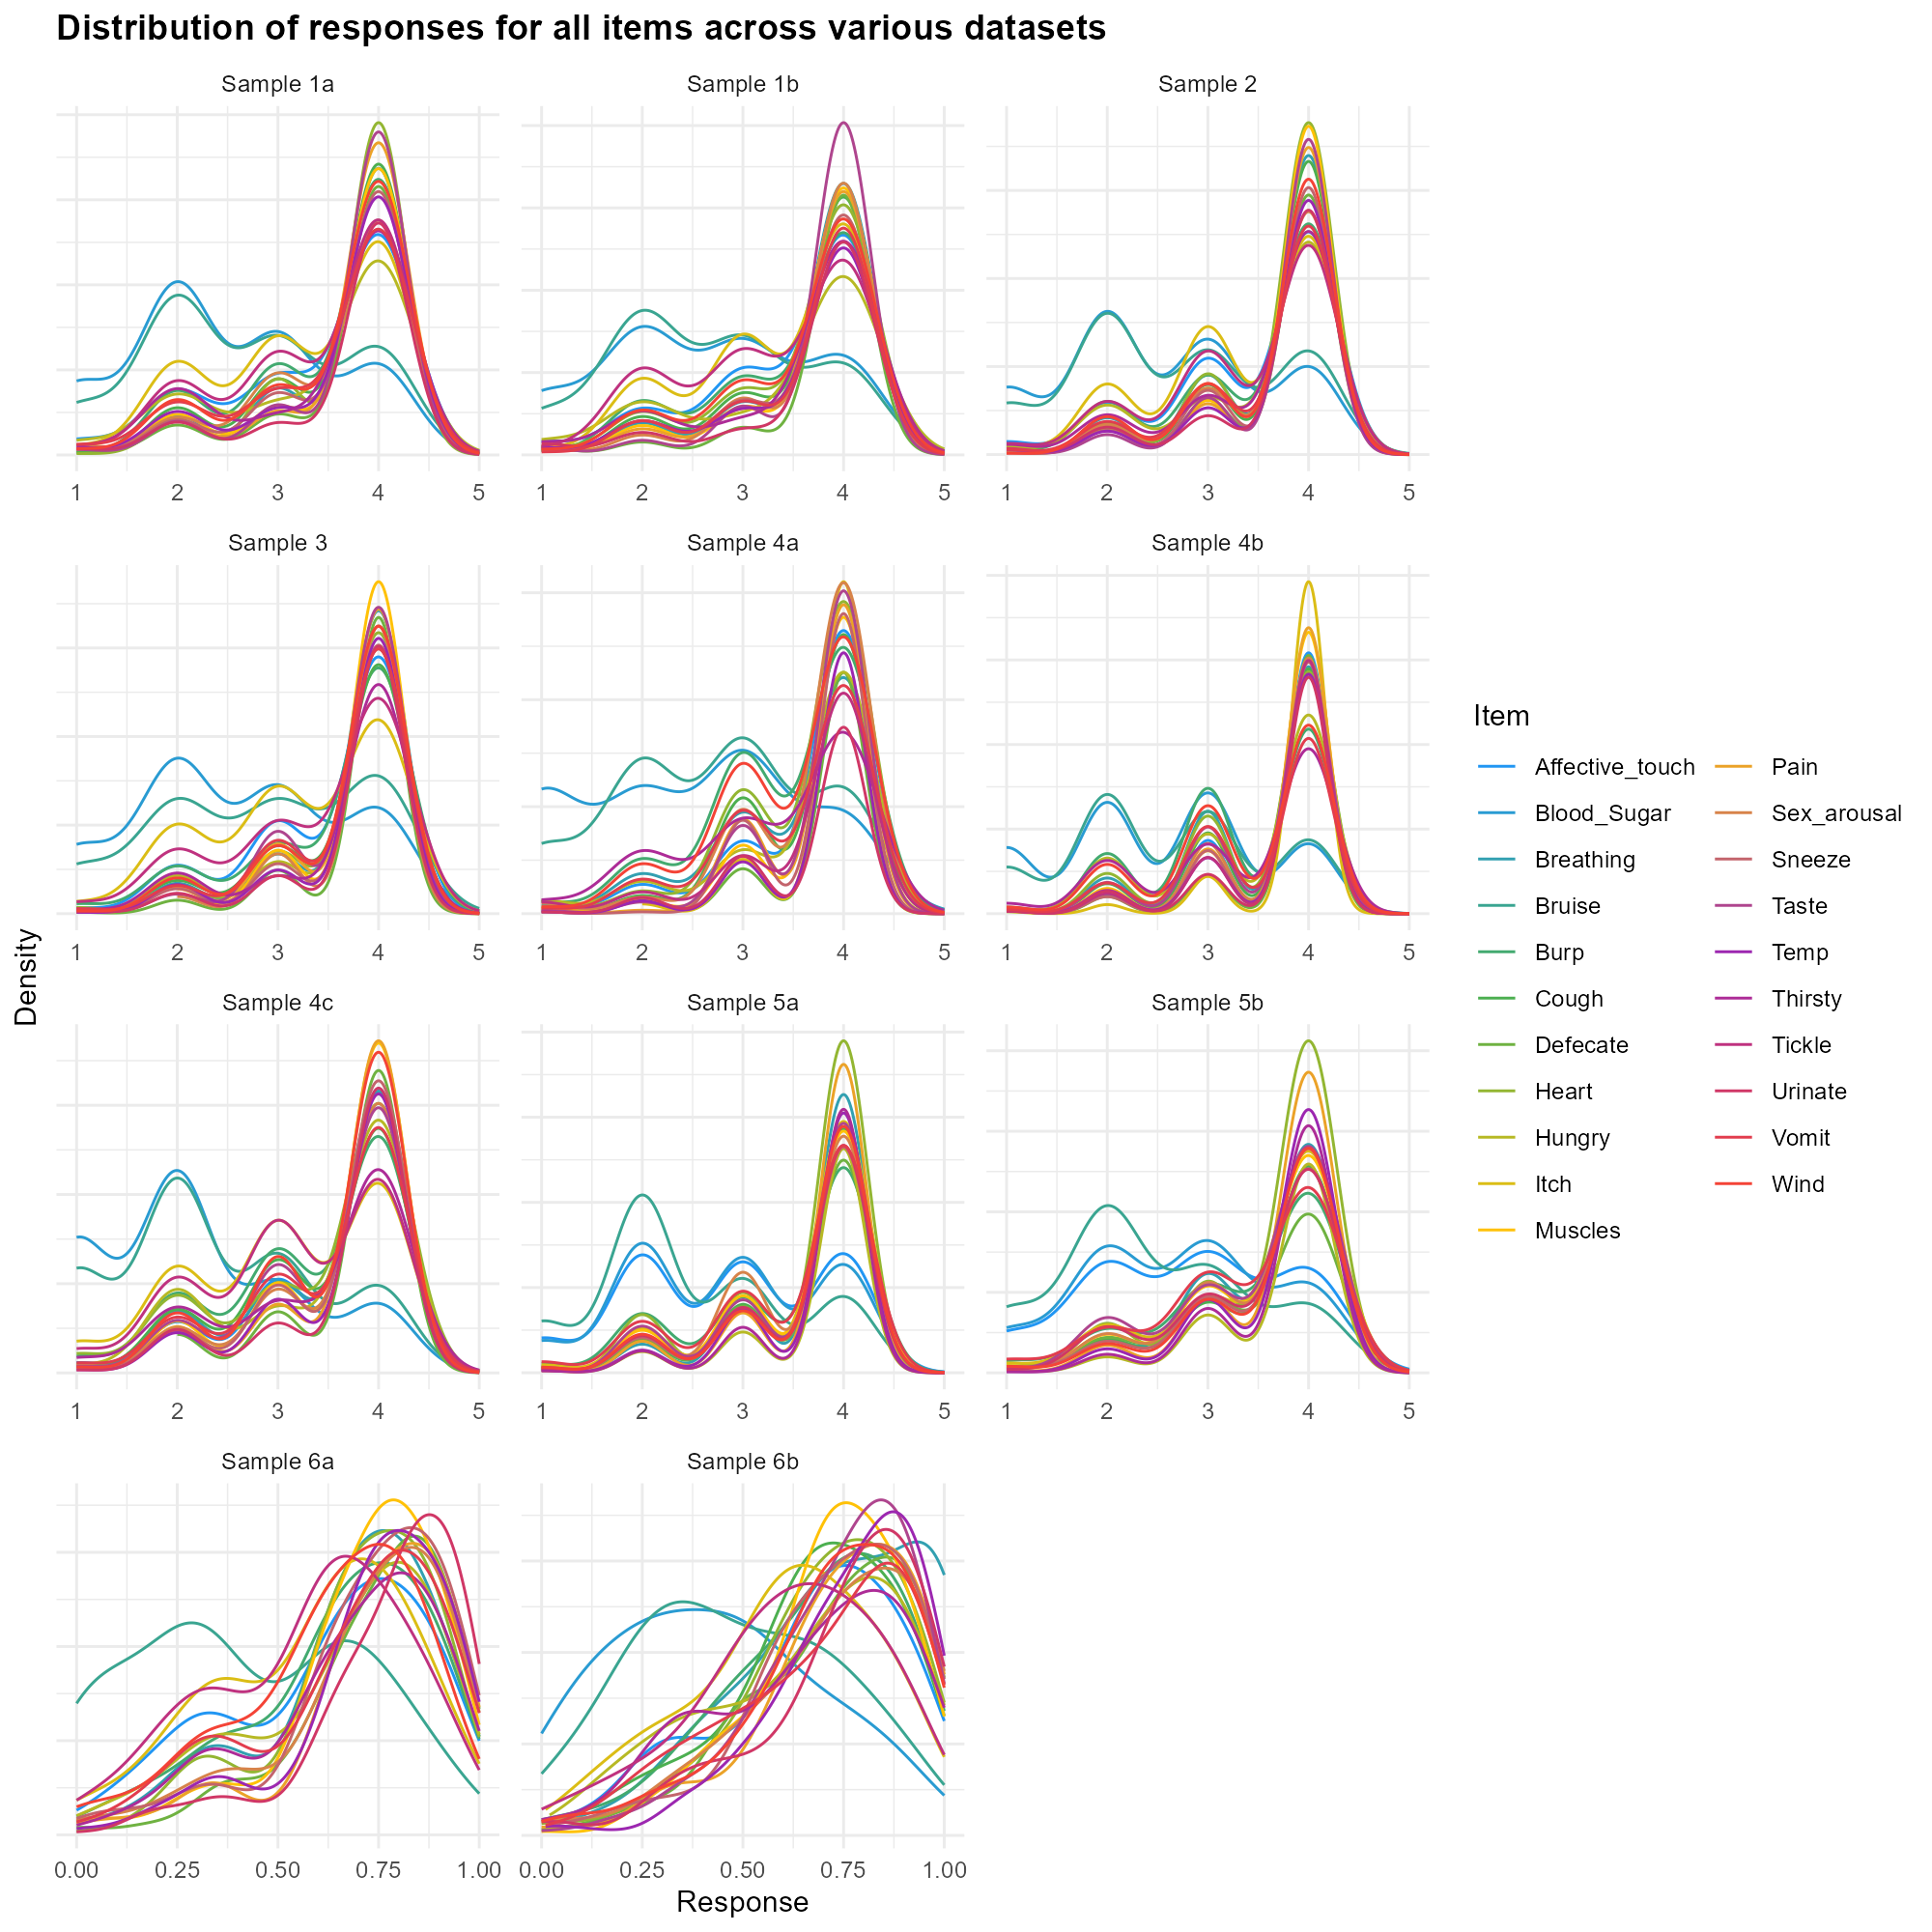
\includegraphics[width=1\linewidth,height=\textheight,keepaspectratio]{../../analysis/figures/Figure1.png}

\end{figure*}

UVA flagged ``itch'' and ``tickle'' as strongly redundant; ``tickle''
was removed from further analyses given its redundancy and absence from
some datasets due to translation issues. Additional pairs were flagged
as moderately redundant (``wind''/``burp''; ``urinate''/``defecate'') or
mildly redundant (``sneeze''/``cough''; ``heart''/``breathing'';
``hungry''/``thirsty''), consistently across most samples.

\subsection{Structure Exploration}\label{structure-exploration}

HCA consistently grouped item pairs and triplets across samples:
``wind''/``burp'', ``sneeze''/``cough'', ``itch''/``bruise'',
``urinate''/``defecate'', and ``pain''/``muscles''/``temperature''. EGA
largely replicated this, with an additional cluster comprising ``sexual
arousal'', ``affective touch'', ``temperature'', ``pain'', ``muscles'',
and ``taste''. EFA suggested an optimal 3-factor solution:
expulsion-related items (``burp'', ``wind'', ``cough'', ``sneeze'',
``vomit''), visceroceptive items (``heart'', ``breathing'', ``hungry'',
``thirsty'', ``urinate'', ``defecate''), and items not directly
accessible via internal sensation alone (``bruise'', ``blood sugar'').
Full results are available via the GitHub repository above.

Initial structural analyses flagged six further problematic items beyond
``tickle'': ``taste'' showed a lone or unstable association pattern;
``affective touch'' exhibited cross-loadings and instability; ``vomit''
was weakly associated with other items; ``itch'' formed no consistent
cluster; and ``temperature'' and ``sexual arousal'' showed redundant but
unreliable associations. These six items, alongside ``tickle'', were
removed, and structural analyses were re-run on the remaining 14 items
(see Figure~\ref{fig-structure}).

\begin{figure*}[!htbp]

{\caption{{Four structure analysis methods (HCA, EGA, EFA, CFA) were
applied and converged on a consistent optimal solution of 14 items
formed seven pairs: Hungry-Thirsty, Bruise-Blood sugar,
Urinate-Defecate, Muscles-Pain, Breathing-Heart, Cough-Sneeze,
Wind-Burp. While EFA suggested 3 factors, CFA confirmed the superiority
of the 7-factor model over alternative
structures.}{\label{fig-structure}}}}

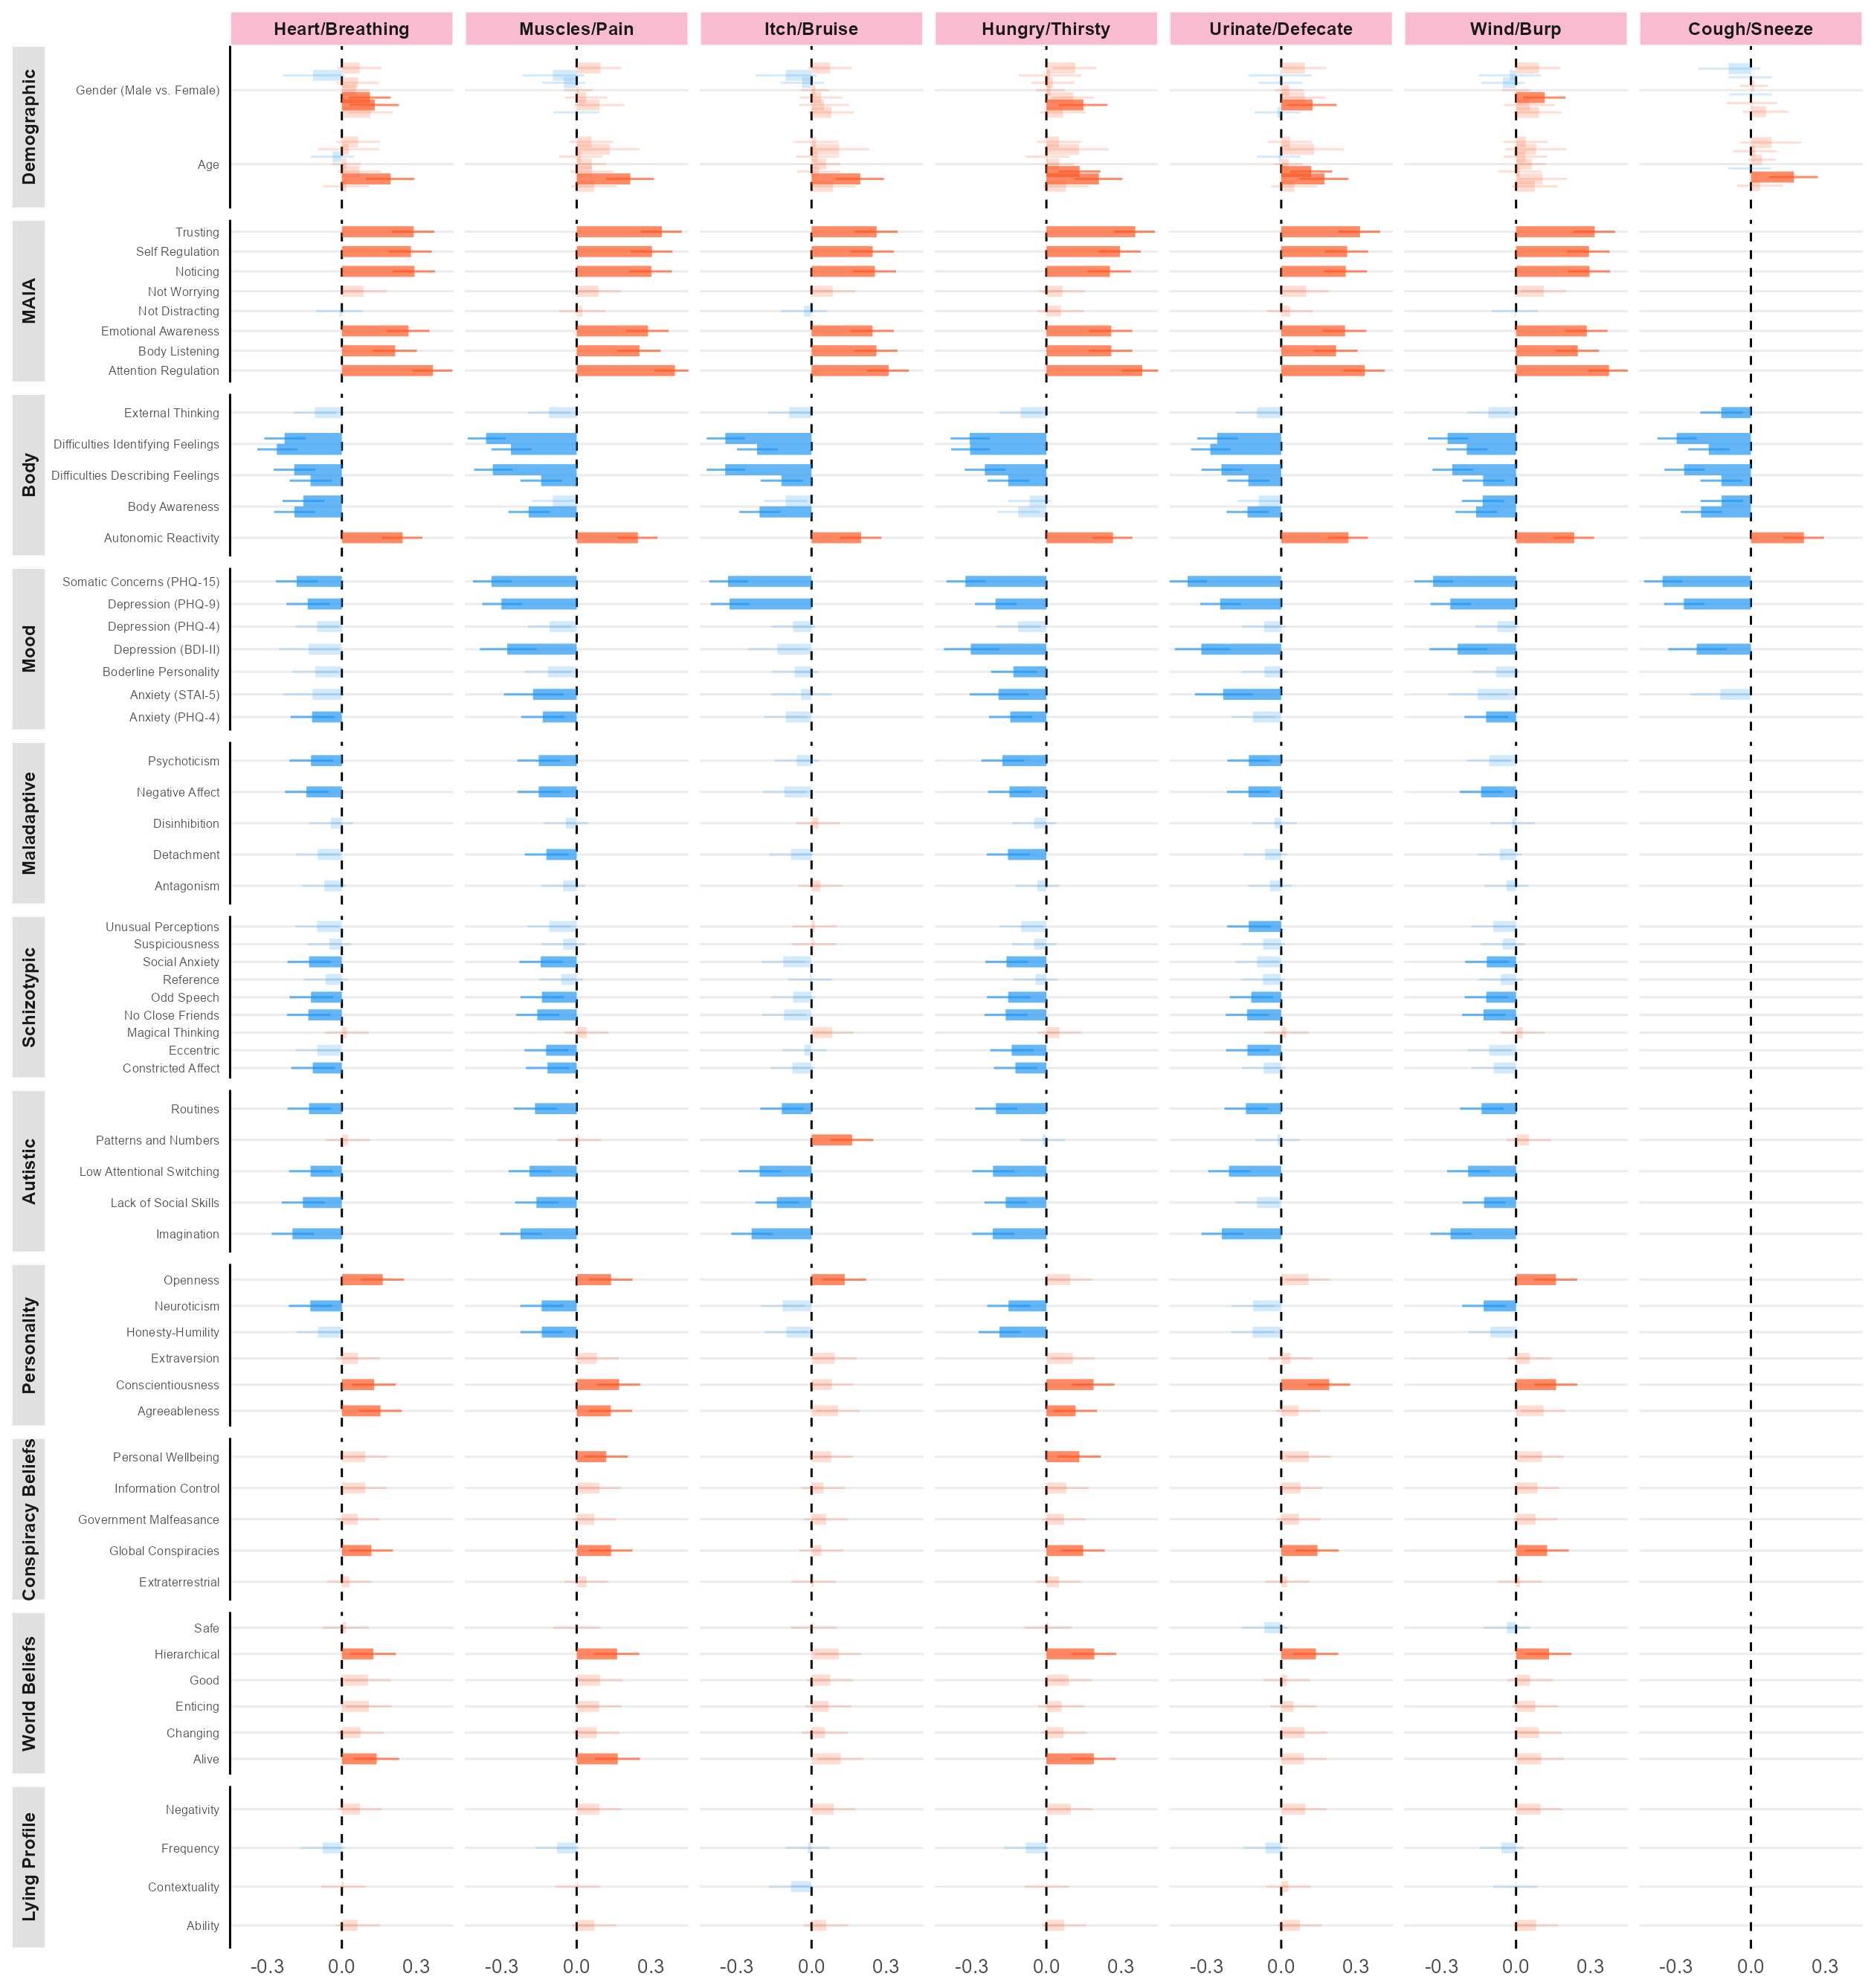
\includegraphics[width=1\linewidth,height=\textheight,keepaspectratio]{../../analysis/figures/Figure2.png}

\end{figure*}

HCA and EGA yielded highly consistent results, identifying seven stable
item pairs: Hungry-Thirsty, Bruise-Blood sugar, Urinate-Defecate,
Muscles-Pain, Breathing-Heart, Cough-Sneeze, and Wind-Burp. HCA
additionally grouped Urinate-Defecate with Muscles-Pain, and the two
expulsion pairs (Wind-Burp, Cough-Sneeze) together. EFA again suggested
a 3-factor solution: expulsion items (``burp'', ``wind'', ``cough'',
``sneeze''), the Urinate-Defecate pair, and the remaining items.

\subsection{Confirmatory Factor Analysis
(CFA)}\label{confirmatory-factor-analysis-cfa}

We used CFA to fit and compare candidate structures from the previous
analyses: a 1-factor (G-model), 3-factor (EFA), 3+1 (EFA + general
factor), 5-factor (HCA), 5+1 (HCA + general factor), 7-factor (EGA), and
7+1 (EGA + general factor) model. The 7-factor EGA model provided the
best fit (RMSEA = 0.035, χ2\chi\^{}2 χ2 = 2,334.112, CFI = 0.984),
followed by EGA + general factor (RMSEA = 0.054, χ2\chi\^{}2 χ2 =
6,876.395, CFI = 0.952) and the 5-factor HCA model (RMSEA = 0.078,
χ2\chi\^{}2 χ2 = 13,441.878, CFI = 0.906). All remaining models
performed poorly (RMSEA \textgreater{} 0.08, CFI \textless{} 0.90). The
EGA model also yielded the lowest BIC; all other models showed
substantially weaker evidence (BIC-based Bayes Factor \textless{}
1/100).

Across individual datasets, the 7-factor EGA model provided the best fit
in 8 of 13 samples where CFA converged. In these samples, the 7-factor
EGA model showed excellent performance, with low RMSEA values (≈
0.025--0.057), high CFI values (≥ 0.95), and substantially lower χ2
values compared to alternative models. Adding a general factor improved
fit in three samples for which the 7-factor EGA + general factor model
showed acceptable RMSEA (≈ 0.048--0.061) and CFI (≈ 0.929--0.957)
values. The 5-factor + general factor model was preferred in two (RMSEA
= 0.049/0.057, CFI = 0.955/0.919). Bayes factor comparisons aligned with
BIC-based conclusions. Overall, while the EGA model was preferred in
most samples, bifactor models provided some evidence for a common IAS
factor.

\subsection{Discussion}\label{discussion}

Study 1 aimed to systematically evaluate the structure of the IAS using
a mega-analytic approach with both factor-analytic and network-based
methods. Previous research has highlightd inconsistencies in optimal
factor structure {[}e.g., unidimensional, bifactor, and two-factor
solutions; Brand et al. (\citeproc{ref-brand2023}{2023}); Campos et al.
(\citeproc{ref-campos2021}{2021}); Lin et al.
(\citeproc{ref-lin2023}{2023}); Murphy et al.
(\citeproc{ref-murphy2019}{2019}); Koike and Nomura
(\citeproc{ref-koike2023}{2023}){]} and raised concerns about specific
items (e.g., low discrimination, local dependencies, items less
accessible to interoception). To address these concerns and issues, we
combined 17 datasets with over 33,000 participants, to provide the most
comprehensive analysis of IAS structure to date, across both combined
and individual datasets. We conducted analyses across both combined and
individual datasets, allowing an examination of overall and
dataset-specific results and how they compared across three different
structural analysis methods (EFA, HCA, EGA).

Seven item pairs (Hungry-Thirsty, Bruise-Blood Sugar, Urinate-Defecate,
Muscles-Pain, Breathing-Heart, Cough-Sneeze, Wind-Burp) emerged
consistently across datasets and methods, yielding a refined 14-item IAS
with superior fit over alternative models. Rather than measuring a broad
``interoceptive accuracy'' construct, the IAS appears to reflect
clusters of tightly coupled items tied to specific bodily sensations -
both directly felt and inferred or anticipatory (e.g., Bruise-Blood
Sugar). Notably, while \(\chi^2\) and BIC can be sensitive to large
samples, conclusions are further supported by replication across
analytic approaches and individual datasets.

Alternatively, item pairings may also reflect shared temporal or
functional characteristics. For instance, Cough-Sneeze and Wind-Burp
involve rapid reflexive responses and frequent co-occurrence, while
Hungry-Thirsty and Urinate-Defecate reflect homeostatic regulation and
recurrent need states, potentially eliciting similar response strategies
despite distinct underlying physiology. These explanations need not
exclude interpretation of pairings as intuitive bodily domains (e.g.,
visceral, expulsion, musculoskeletal). Indeed, temporal and functional
similarities are themselves grounded in bodily organisation, suggesting
multiple overlapping sources of structure. This convergence contribute
to the intuitive coherence of the item pairs while also increasing
redundancy and instability when weakly discriminating items are
retained, thereby complicating factor-analytic solutions and likely
contributing to inconsistencies in prior findings
(\citeproc{ref-campos2021}{Campos et al., 2021};
\citeproc{ref-lin2023}{Lin et al., 2023}).

Study 1 findings highlight the need for targeted scale refinement and
context-sensitive interoception measures. Many bodily sensations are
inherently ambiguous (e.g., a racing heart may signal exertion, anxiety,
or excitement), making it unclear which state participants reference
when responding. Such ambiguity likely constrains ecological validity
and contributes to cross-study variability; context-specific phrasing
may therefore be necessary to more accurately capture interoceptive
beliefs and reduce measurement noise
(\citeproc{ref-makowski2025mint}{Makowski, Neves, et al., 2025}; e.g.,
\citeproc{ref-vlemincx2023novel}{Vlemincx et al., 2023}).

Overall, Study 1 suggests that, after removal of problematic items the
IAS is best conceptualized as a set of item clusters rather than a
unidimensional scale. This structural insight forms the foundation for
Study 2, where dispositional correlates are examined to further evaluate
the IAS's construct validity.

\section{Study 2}\label{study-2}

Although widely adopted, evidence on the IAS's associations with
personality traits, affective dispositions, and related constructs
remains scattered and inconsistent (\citeproc{ref-brand2023}{Brand et
al., 2023}; \citeproc{ref-lin2023}{Lin et al., 2023};
\citeproc{ref-murphy2019}{Murphy et al., 2019};
\citeproc{ref-todd2022}{Todd et al., 2022}). In Study 2 we aimed to
provide a robust overview of the dispositional correlates of the IAS by
leveraging and combining a large number of available datasets containing
both the IAS, other measures of interoception, and dispositional
correlates. We also sought to assess whether structural improvements of
the 14-item IAS translate into clearer, more interpretable, and more
reliable external associations by comparing associations to
dispositional variables with the original 21-item unidimensional
solution, offering a more efficient alternative to the longer version
for future research.

\subsection{Methods}\label{methods-1}

\subsubsection{Materials}\label{materials}

We selected measures appearing in at least one Study 1 dataset and/or
relevant to the study scope (physiology, mood, personality,
psychopathological and neurodevelopmental traits, and beliefs). Where
applicable, regular and abridged scale versions were merged (e.g., the
2-item GAD and PHQ measures were combined into the PHQ-4).

\paragraph{Interoception and Interoception Related
Measures.}\label{interoception-and-interoception-related-measures}

Interoception-related measures included the Multidimensional Assessment
of Interoceptive Awareness Version-2 (MAIA-2,
\citeproc{ref-mehling2018multidimensional}{Mehling et al., 2018}), the
Body Perception Questionnaire Short Form (BPQ-SF,
\citeproc{ref-cabrera2018assessing}{Cabrera et al., 2018}), and the
Interoceptive Confusion Questionnaire (ICQ,
\citeproc{ref-brewer2016alexithymia}{Brewer et al., 2016}). We also
included the Bermond--Vorst Alexithymia Questionnaire (BVAQ,
\citeproc{ref-vorst2001validity}{Vorst \& Bermond, 2001}), and the
Toronto Alexithymia Scale (TAS-20, \citeproc{ref-bagby1994twenty}{Bagby
et al., 1994}), due to the close relationship between interoception
deficits and alexithymia (e.g.,
\citeproc{ref-brewer2016alexithymia}{Brewer et al., 2016};
\citeproc{ref-gaggero2021}{Gaggero et al., 2021}).

\paragraph{Mood and Anxiety Related
Measures.}\label{mood-and-anxiety-related-measures}

Scores from depression and anxiety-related measures were included due to
their established associations with interoceptive processing
(\citeproc{ref-khalsa2018}{Khalsa, Adolphs, Cameron, Critchley,
Davenport, Feinstein, Feusner, Garfinkel, Lane, Mehling, Meuret, et al.,
2018}); namely the Patient Health Questionnaire-4 (PHQ-4,
\citeproc{ref-kroenke2009ultra}{Kroenke et al., 2009}), the Patient
Health Questionnaire-15 (PHQ-15, \citeproc{ref-kroenke2002phq}{Kroenke
et al., 2002}), the Patient Health Questionnaire-9 (PHQ-9,
\citeproc{ref-kroenke2001phq}{Kroenke et al., 2001}), the Short Mood and
Feelings Questionnaire (MFQ, \citeproc{ref-angold1995development}{Angold
et al., 1995}), the Beck Depression Inventory-II (BDI-II,
\citeproc{ref-beck1996beck}{Beck et al., 1996}), the State--Trait
Anxiety Inventory Trait Version (STAI-T,
\citeproc{ref-spielberger1970manual}{Spielberger, 1970}; and STAIT-T,
\citeproc{ref-zsido2020development}{Zsido et al., 2020}), the
Generalized Anxiety Disorder Scale (GAD-7,
\citeproc{ref-spitzer2006brief}{Spitzer et al., 2006}), and General
Anxiety Disorder-2 (GAD-2, \citeproc{ref-kroenke2007anxiety}{Kroenke et
al., 2007}, obtained from the PHQ-4).

\paragraph{Psychopathological and Neurodevelopmental
Traits.}\label{psychopathological-and-neurodevelopmental-traits}

Dimensional psychopathological and neurodevelopmental-related trait
scores were included from the Personality Inventory for DSM-5 Short Form
(PID-5-SF, \citeproc{ref-thimm2016personality}{Thimm et al., 2016}), the
Autism Spectrum Quotient Short Form (ASQ-S,
\citeproc{ref-hoekstra2011construction}{Hoekstra et al., 2011}), the
Schizotypal Personality Questionnaire -- Brief Revised (SPQ-BR,
\citeproc{ref-davidson2016schizotypal}{Davidson et al., 2016}), and the
McLean Screening Instrument for Borderline Personality Disorder
(MSI-BPD, \citeproc{ref-zanarini2003zanarini}{Zanarini, 2003}).

\paragraph{Personality.}\label{personality}

Personality-related measures included the NEO Five-Factor Inventory,
Neuroticism subscale (NEO-FFI, \citeproc{ref-costa1992personality}{Costa
et al., 1992}), the Mini International Personality Item Pool
(MINI-IPIP6, \citeproc{ref-sibley2011mini}{Sibley et al., 2011}), and
the Big Five Inventory Short Form (BFI-S,
\citeproc{ref-rammstedt2007measuring}{Rammstedt \& John, 2007}).

\paragraph{Beliefs and Misbeliefs.}\label{beliefs-and-misbeliefs}

Beliefs- and misbeliefs-related measures included the Lie Scale (LIE,
\citeproc{ref-makowski2023structure}{Makowski et al., 2023}), the
Generic Conspiracist Beliefs Scale (GCBS,
\citeproc{ref-brotherton2013measuring}{Brotherton et al., 2013}), and
the Primal World Beliefs Inventory (PI-99,
\citeproc{ref-clifton2019primal}{Clifton et al., 2019}) and its short
form (PI-18, \citeproc{ref-clifton2021brief}{Clifton \& Yaden, 2021}).
These instruments assess individual differences in conspiracist, world,
and lying beliefs. This domain represents a novel avenue of research in
the context of interoception, as such beliefs have not been previously
assessed in relation to interoceptive processes.

\subsubsection{Data Analysis}\label{data-analysis-1}

\begin{figure*}[!htbp]

{\caption{{Meta-analytic associations (95\% CI of standardised
coefficients) between the IAS (total score and seven item pairs) and
dispositional measures across 17 open-access datasets. Positive
associations are shown in red, negative associations in blue.
Non-significant associations (CI crossing zero) are transparent. The
IAS-21 showed positive associations with most MAIA facets and BPQ-Body
Awareness, negative associations with interoceptive deficit measures
(TAS, ICQ), negative associations with the BPQ-Autonomic Reactivity,
moderate negative associations with mood measures, and weaker, more
selective associations with psychopathological and neurodevelopmental
traits and belief measures. Certain item pairings, particularly
Hungry--Thirsty and Bruise--Blood sugar, drove the strongest effects,
highlighting domain-specific patterns in self-perceived interoceptive
accuracy.}{\label{fig-correlations}}}}

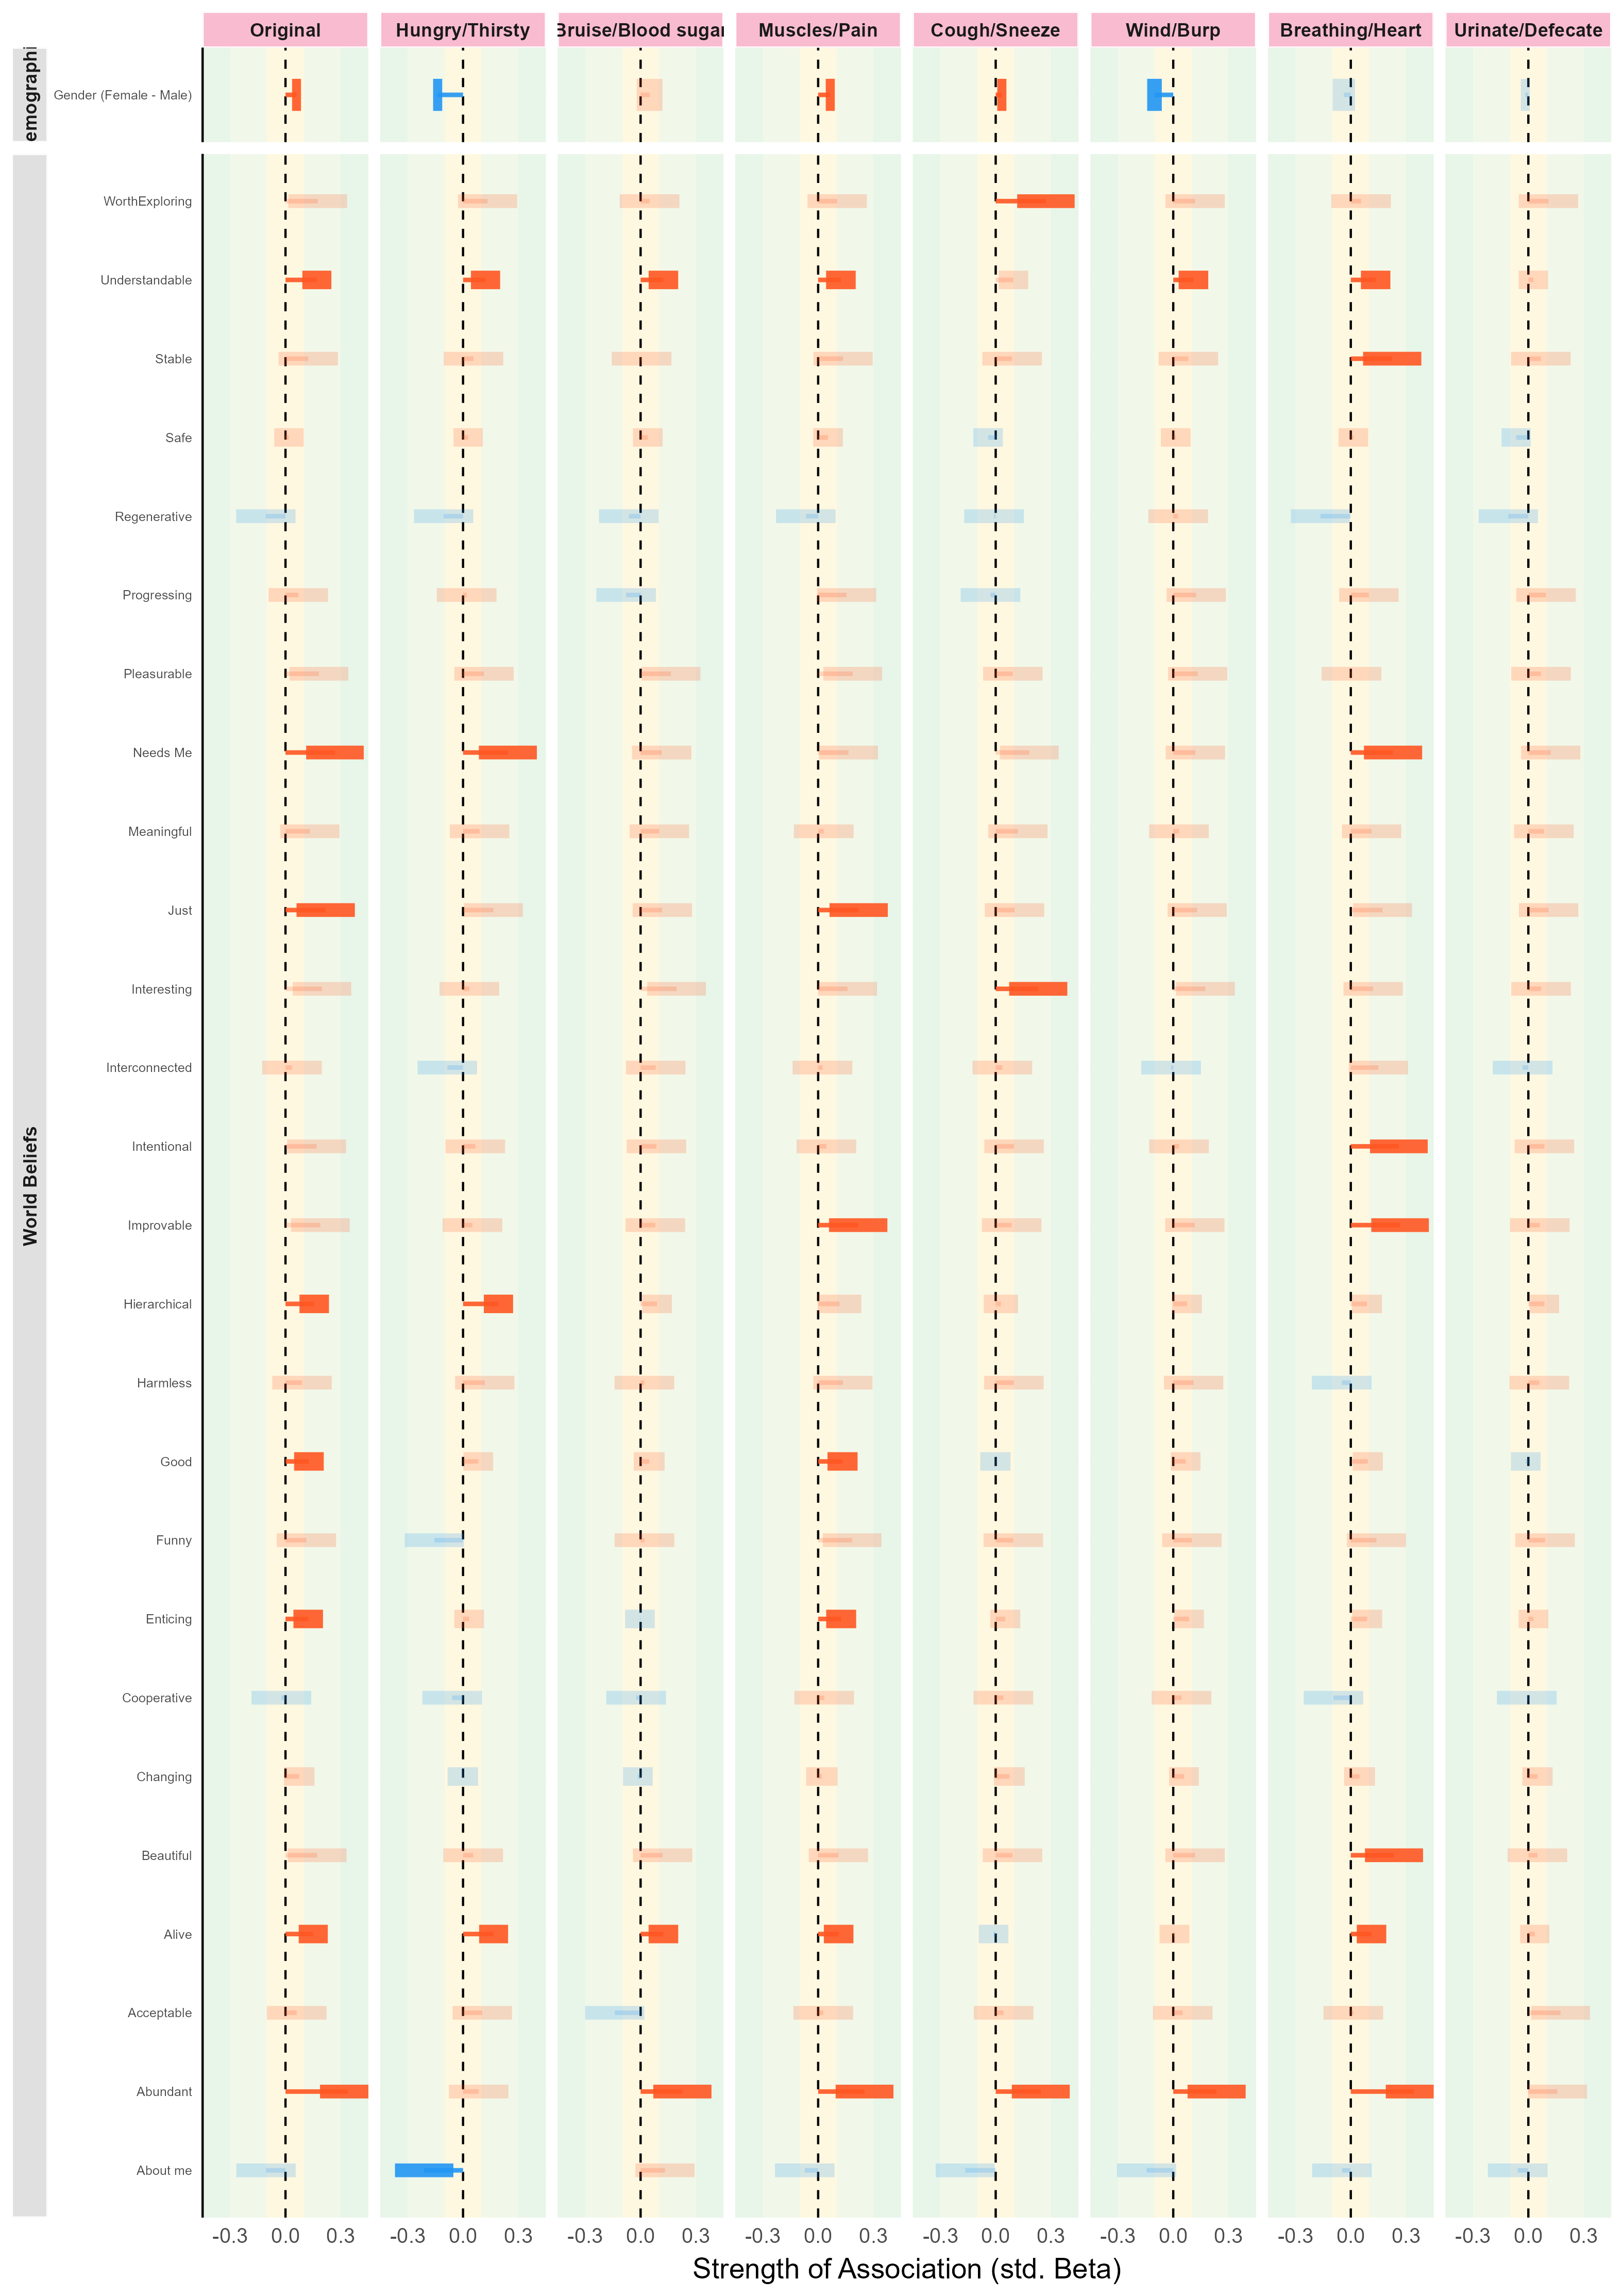
\includegraphics[width=1\linewidth,height=\textheight,keepaspectratio]{../../analysis/figures/Figure3.png}

\end{figure*}

All variables were extracted and standardised (z-scored) for the
aggregated dataset. Scores were harmonised where meaningful (e.g., the
18-item and 99-item PI versions were combined) and missing data were
excluded per-model to maximise statistical power.

Akin to a meta-analytic framework, datasets were treated as clusters
(random groups), and pooled estimates of the associations that account
for both within- and between-sample variability were computed. This
approach allowed for the estimation of multiple associations while still
accounting for study heterogeneity and intra-study uncertainty (i.e.,
measurement uncertainty within the studies). Specifically, associations
were estimated using mixed models via the \emph{glmmTMB} package
(\citeproc{ref-glmTMB}{McGillycuddy et al., 2025}), postprocessed with
the easystats ecosystem (\citeproc{ref-ben2020effectsize}{Ben-Shachar et
al., 2020}; \citeproc{ref-ludecke2020extracting}{Lüdecke et al., 2020};
\citeproc{ref-makowski2025modelbased}{Makowski, Ben-Shachar, et al.,
2025}). Each predictor was entered separately with the seven IAS item
pairs from Study 1 (Hungry--Thirsty, Muscles--Pain, Wind--Burp,
Urinate--Defecate, Breathing--Heart, Bruise--Blood Sugar, Cough--Sneeze)
and the original IAS total score as outcomes, with dataset as a random
intercept and predictor as a random slope. Given the large sample size,
we focus on effect sizes and confidence intervals rather than
\emph{p}-values.

From each fitted model, we extracted standardised regression
coefficients (interpretable as a correlation index), and 95\% confidence
intervals (additional details on \emph{p}-values, convergence status,
and sample sizes are available in the GitHub repository). Results are
summarized in Figure~\ref{fig-correlations} and we report the mean
coefficient in the text when consistent across measures.

\subsection{Results}\label{results-1}

\subsubsection{Demographics}\label{demographics}

Age showed consistent positive standardised associations across IAS
correlates (β = .13), including both the IAS total scores and the scores
for the 7-pairs, with all effects significant. Gender displayed
near-zero effects (β = −.06) and was only significant for the
Hungry--Thirsty, Wind--Burp, and Urinate--Defecate pairs.

\subsubsection{Interoception and Interoception Related
Measures}\label{interoception-and-interoception-related-measures-1}

MAIA subscales showed robust positive standardised associations with the
IAS. Noticing had the strongest association (β = .26), followed by
Attention Regulation (β = .25) with other subscales (Body Listening,
Trusting, Emotional Awareness and Self-Regulation) in the .19--.24
range, all significant. Effects were generally strongest for the full
IAS, except for Body Listening, which peaked for the Bruise--Blood sugar
pair. Not Distracting was significant only for the full IAS,
Hungry-Thirsty, Bruise-Blood sugar and the Muscles-Pain pairs, albeit
weakly (β ≈ −.02 to .06). Not Worrying was significant only for the full
IAS and the Hungry--Thirsty and Urinate--Defecate pairs (β ≈ −.01 to
.04).

The BPQ's Autonomic Reactivity subscale was reliably negatively
associated across the seven item pairs (β = −.19), reaching significance
for all pairs except Bruise--Blood sugar and Breathing--Heart. In
contrast, the Body Awareness subscale of the BPQ was positive and
significant across most pairs (β = .15; range = .10 to .22) except for
Wind-Burp and Urinate-Defecate.

Interoceptive deficits showed consistent negative associations:
Alexithymia measures (TAS, BVAQ) were robustly negative (β ≈ −.13 to
−.2), except for the BVAQ Affective subscale, which was positive for
Bruise--Blood sugar (β = .16). Interoceptive confusion (ICQ) was also
negative across all IAS measures (β = −.32; range = −.49 to −.20).

\subsubsection{Mood and Anxiety Related
Measures}\label{mood-and-anxiety-related-measures-1}

Depression (β = −.20) and anxiety (β = −.20) showed consistent negative
associations across the IAS and all its pairs, with the strongest
effects observed for the Hungry--Thirsty dimension. However, looking at
specific measures revealed some differences.

The MFQ was largely nonsignificant except for a negative association
with Breathing--Heart, while somatic concerns (PHQ-15) were unrelated to
the IAS total scale but had weak negative associations with the
Hungry--Thirsty, Bruise--Blood sugar, and Urinate--Defecate pairs (from
−.22 to −.05).

Other mood indices (PHQ-9, PHQ-4, GAD-7) produced generally weaker but
often reliable negative coefficients (typically −.10 to −.15), though
effects sometimes appeared only for specific pairs (e.g., PHQ-4 was
significant for all pairs except Wind--Burp and Breathing--Heart).
Across anxiety and depression measures, the Hungry--Thirsty pair
consistently had the strongest standardised effects.

\subsubsection{Psychopathological and Neurodevelopmental
Traits}\label{psychopathological-and-neurodevelopmental-traits-1}

Psychopathological traits were generally negatively associated with the
IAS scores. Detachment, Psychoticism, and Negative Affect demonstrated
the most reliable, albeit weak, negative associations with IAS scores
(from −.08 to −.10), again primarily driven by the Hungry--Thirsty,
Bruise--Blood sugar, and Muscles--Pain pairs.

Other maladaptive traits were unrelated to IAS scores. Notably,
Antagonism showed a significant positive association, limited to the
Bruise--Blood sugar pair (β = .14), whereas Borderline Personality was
uniquely negatively associated with Hungry--Thirsty (β = −.14).

A comparable trend was observed for autistic traits (ASQ), with the
strongest effects driven by the Hungry--Thirsty, Bruise--Blood sugar,
and Muscles--Pain pairs, which yielded the largest negative
coefficients. Among ASQ subscales, Imagination (β = −.18) exhibited the
most consistent pattern of negative associations across pairs except for
Cough--Sneeze.

Schizotypal traits showed a similarly negative pattern of associations
to IAS scores. Social Anxiety (β = −.11) and No Close Friends (β = −.12)
displayed the most consistent effects. Although some facets were
unrelated to the total IAS score, they were associated with specific
item pairs: Unusual Perceptions with Muscles--Pain and
Urinate--Defecate, and Eccentric with Hungry--Thirsty and
Urinate--Defecate.

\subsubsection{Personality}\label{personality-1}

Among the Big Five traits, Openness (β = .10), Agreeableness (β = .08),
and Conscientiousness (β = .11) exhibited small yet consistent positive
associations, most clearly for the total IAS score. Extraversion showed
a weak but positive association, driven primarily by the Bruise--Blood
sugar pair (β = .17). In contrast, Honesty--Humility (β = −.10) had a
small negative effect, most clearly for the Hungry--Thirsty and
Bruise--Blood sugar pairs. Finally, Neuroticism (β = −.23) was
negatively associated with the IAS, with the strongest effect observed
for the Hungry--Thirsty pair (β = −.22).

\subsubsection{Beliefs and Misbeliefs}\label{beliefs-and-misbeliefs-1}

Within the Lying Profile, only Lying Contextuality showed a modest
negative coefficient for Bruise--Blood sugar (β = −.12). Global
Conspiracies (GCBS) beliefs were associated with the total IAS and three
pairs (β = .10): Hungry--Thirsty, Cough-Sneeze and Urinate-Defecate.
Primal world beliefs were largely null, with small positive associations
for appraising the world as being ``Understandable'', ``Alive'', and
``Hierarchical'', with Hungry--Thirsty (β = .09). Appraising the world
as ``Good'' was uniquely positively related with Muscles--Pain (β =
.09).\\
Overall, the original IAS total score had the greatest number of
significant standardised effects (28), though many were driven by
specific item pairs rather than uniform scale-wide associations.
Hungry--Thirsty (17) and Bruise--Blood sugar (10) consistently yielded
the largest standardised coefficients, especially for interoception,
mood, and psychopathological and neurodevelopmental trait measures.
Other item pairs (Cough--Sneeze, Wind--Burp, Urinate--Defecate)
contributed little unique variance and rarely had meaningful
standardised effects.

\subsection{Discussion}\label{discussion-1}

Using a meta-analytical approach across 17 datasets, Study 2 examined
the dispositional correlates of the IAS and whether the refined 14-item
version translated into clearer and more reliable associations than the
original 21-item scale.

The IAS showed positive associations with all MAIA facets except
Not-Distracting and Not-Worrying, replicating prior findings
(\citeproc{ref-brand2023}{Brand et al., 2023};
\citeproc{ref-todd2022}{Todd et al., 2022}), and positive associations
with the BPQ Body Awareness subscale, consistent with previous research
(\citeproc{ref-brand2023}{Brand et al., 2023};
\citeproc{ref-gaggero2021}{Gaggero et al., 2021};
\citeproc{ref-koike2023}{Koike \& Nomura, 2023}). Autonomic reactivity
indices were more strongly and negatively associated with IAS scores,
supporting earlier observations that reactivity may reflect bodily
signal processing captured by self-reported interoceptive accuracy
(\citeproc{ref-todd2022}{Todd et al., 2022}). Measures of interoceptive
difficulties --- alexithymia and interoceptive confusion --- were
negatively associated with IAS scores, consistent with prior work
(\citeproc{ref-brand2023}{Brand et al., 2023};
\citeproc{ref-koike2023}{Koike \& Nomura, 2023};
\citeproc{ref-lin2023}{Lin et al., 2023};
\citeproc{ref-murphy2019}{Murphy et al., 2019}).

Although the BPQ Body Awareness--IAS association replicates some
findings, others have reported null (\citeproc{ref-murphy2019}{Murphy et
al., 2019}), negative (\citeproc{ref-lin2023}{Lin et al., 2023}), or
even quadratic relationships (\citeproc{ref-campos2021}{Campos et al.,
2021}). Mixed findings may reflect inconsistent interpretations of BPQ
items; specifically, whether they capture attentional focus or perceived
detection accuracy (\citeproc{ref-campos2021}{Campos et al., 2021};
\citeproc{ref-gabriele2022dissociations}{Gabriele et al., 2022}) and
should therefore be interpreted cautiously. Future studies should assess
participants' understanding of BPQ items to clarify this relationship.

Across mood measures, most item pairs showed small-to-moderate
associations, indicating shared variance between interoceptive
self-reports and affective tendencies (\citeproc{ref-koike2023}{Koike \&
Nomura, 2023}; \citeproc{ref-murphy2019}{Murphy et al., 2019}).
Associations with psychopathological and neurodevelopmental traits were
more selective, with negative effects concentrated in visceral pairings
(Hungry--Thirsty, Bruise--Blood Sugar), suggesting self-reported
interoceptive accuracy for visceral sensations is more strongly linked
to affective and clinical traits than accuracy for somatic or
respiratory reflexes.

Personality associations followed a similar domain-specific pattern.
Extraversion was most strongly associated with Bruise--Blood Sugar,
Neuroticism and Honesty--Humility with Hungry--Thirsty, and Openness,
Conscientiousness, and Agreeableness with the full scale. These results
partially align with prior work (\citeproc{ref-brand2023}{Brand et al.,
2023}) but require replication, as well as evaluation of associations
involving other personality traits. Overall, these results suggest that
IAS--personality associations depend on the bodily domain represented.

Associations with belief systems were uniformly small. Weak positive
associations emerged with certain primal world beliefs (e.g., perceiving
the world as comprehensible or alive) and selected conspiracy belief
dimensions (Global Conspiracies, Personal Wellbeing), concentrated in
Hungry--Thirsty and Bruise--Blood Sugar pairs. This suggests links
between interoceptive self-report and broader cognitive or worldview
constructs are modest and domain-specific.

Notably, this study prioritised general patterns across aggregated
datasets rather than systematic between-sample differences;
dataset-specific effects were not examined in detail. Although
cross-sample variability is reflected in estimate uncertainty, future
research could profitably investigate sample-specific associations and
the causes of divergences across datasets.

In summary, the 14-item IAS performed comparably to the original 21-item
version across mood, psychopathological, neurodevelopmental, and
interoceptive measures. However, associations were often non-uniform
across bodily domains, driven primarily by specific item pairs ---
particularly Hungry--Thirsty and Bruise--Blood Sugar, which showed the
strongest and most consistent associations with interoceptive,
affective, and personality measures. Other pairs contributed little
unique information, especially for psychopathological,
neurodevelopmental, and belief measures. The homeostatic salience of
Hungry--Thirsty and the contextual relevance and visual/psychological
prominence of Bruise--Blood Sugar may underlie their stronger
dispositional associations.

Overall, findings support the validity of the original IAS general score
while positioning the refined 14-item scale as a more efficient and
interpretively nuanced alternative.

\section{General Discussion}\label{general-discussion}

Across two studies, we used a mega-analytic approach combining data from
17 datasets with over 33,000 participants to provide the most
comprehensive evaluation to date of the IAS, including both its
structure (Study 1) and dispositional correlates (Study 2). These
studies offer new insights into the conceptual interpretation and
practical applications of the IAS, with suggestions for how researchers
may use the IAS in future research.

Study 1 challenges interpretations of the IAS as a single latent
construct (\citeproc{ref-brand2023}{Brand et al., 2023};
\citeproc{ref-murphy2019}{Murphy et al., 2019}), instead suggesting it
captures multiple domain-specific clusters of bodily sensations. Seven
stable item pairs (Hungry--Thirsty, Urinate--Defecate, Muscles--Pain,
Breathing--Heart, Cough--Sneeze, Wind--Burp, Bruise--Blood Sugar)
yielded a refined 14-item structure with superior fit and cross-dataset
stability over unidimensional or bifactor models. Redundant or unstable
items (e.g., Tickle, Taste, Affective Touch) likely weaken
interpretability and contribute to prior inconsistencies
(\citeproc{ref-campos2021}{Campos et al., 2021};
\citeproc{ref-lin2023}{Lin et al., 2023}). Unlike Lin et al.
(\citeproc{ref-lin2023}{2023}), whose 12-item solution supported
unidimensionality, we interpret local dependencies as reflecting
meaningful coupling among functionally related signals (e.g.,
Heart--Breathing) --- mirroring the physiological or phenomenological
co-occurrence of bodily sensations (e.g., hunger with thirst, coughing
with sneezing). Perceived accuracy in one bodily system may thus
generalise to linked sensations, yielding clustered rather than
continuous interoceptive beliefs.

Consistent with this, self-reported interoceptive abilities across
related bodily axes (e.g., cardiac and respiratory) show positive
associations (\citeproc{ref-garfinkel2016interoceptive}{Garfinkel et
al., 2016}), whereas objective measures of interoceptive accuracy across
modalities typically show weak or absent correlations
(\citeproc{ref-banellis2026interoceptive}{Banellis et al., 2026};
\citeproc{ref-bruni2023interoception}{Bruni, 2023};
\citeproc{ref-ferentzi2018interoceptive}{Ferentzi et al., 2018}). This
dissociation suggests that objective interoceptive performance may be
largely domain-specific while subjective beliefs generalise across
functionally related systems. We therefore interpret the present
clustering as reflecting the conceptual organisation of interoceptive
beliefs structured by perceived bodily interdependence, rather than a
single general interoceptive capacity.

Study 2 examined the IAS's associations with interoceptive, affective,
personality, and belief-related traits. Consistent with prior research,
the IAS correlated positively with adaptive interoceptive sensibility
(e.g., MAIA noticing, attention regulation, and body trusting subscales)
and negatively with interoceptive difficulties such as alexithymia and
interoceptive confusion (\citeproc{ref-brand2023}{Brand et al., 2023};
\citeproc{ref-gaggero2021}{Gaggero et al., 2021};
\citeproc{ref-garfinkel2015knowing}{Garfinkel et al., 2015}).

Also consistent with prior research, higher depression and anxiety
symptoms were associated with lower perceived interoceptive accuracy
(\citeproc{ref-brand2023}{Brand et al., 2023};
\citeproc{ref-khalsa2018}{Khalsa, Adolphs, Cameron, Critchley,
Davenport, Feinstein, Feusner, Garfinkel, Lane, Mehling, Meuret, et al.,
2018}; \citeproc{ref-nord2022interoceptive}{Nord \& Garfinkel, 2022}).
Crucially, these associations were not uniform across bodily domains:
the strongest effects involved drive-states (hunger, thirst), while
cardiorespiratory and expulsion domains showed weaker or inconsistent
relationships. This domain specificity suggests that beliefs about
gastrointestinal accuracy may be more psychologically and clinically
relevant than beliefs about reflexive or surface sensations, or that
these signals are more salient and easier to appraise, yielding greater
inter-individual variation.

Domain-specific links to anxiety and depression may help explain
inconsistencies in the interoception--emotion literature.
Performance-based measures of interoceptive accuracy, typically
cardioception, show weak or absent correlations with depression and
anxiety (\citeproc{ref-adams2022association}{Adams et al., 2022};
\citeproc{ref-banellis2025interoceptive}{Banellis et al., 2025};
\citeproc{ref-jenkinson2024interoception}{Jenkinson et al., 2024}),
whereas self-reported measures spanning multiple bodily domains show
stronger negative associations with internalising traits
(\citeproc{ref-brand2022}{Brand et al., 2022};
\citeproc{ref-clemente2024relationship}{Clemente et al., 2024};
\citeproc{ref-lin2023}{Lin et al., 2023}). This discrepancy likely
reflects both conceptual distinctions between perceptual accuracy and
metacognitive beliefs (\citeproc{ref-garfinkel2015knowing}{Garfinkel et
al., 2015}; \citeproc{ref-khalsa2018}{Khalsa, Adolphs, Cameron,
Critchley, Davenport, Feinstein, Feusner, Garfinkel, Lane, Mehling,
Meuret, et al., 2018}; \citeproc{ref-suksasilp2022towards}{Suksasilp \&
Garfinkel, 2022}) and variation in bodily domains assessed. Study 2
extends this by showing that interoceptive belief--affect associations
concentrate in psychologically salient visceral domains, suggesting the
field's reliance on cardioceptive tasks may have obscured meaningful
relationships between affective traits and other interoceptive
modalities.

Similar but weaker patterns emerged for autistic traits, schizotypy, and
maladaptive personality dimensions, which correlated negatively with
interoceptive accuracy beliefs in visceral and musculoskeletal, but not
other, domains. Rather than reflecting a general interoceptive deficit,
diminished accuracy beliefs in specific domains may contribute to
particular socio-emotional and personality features. This aligns with
prior research linking interoceptive self-beliefs to emotional
awareness, social connectedness, and psychopathology
(\citeproc{ref-brand2022}{Brand et al., 2022};
\citeproc{ref-torregrossa2022interoceptive}{Torregrossa et al., 2022};
\citeproc{ref-williams2023characterizing}{Williams et al., 2023}), and
extends it by showing these associations are domain-specific rather than
global.

Together, Studies 1 and 2 suggest that self-perceived interoceptive
accuracy is a differentiated construct varying systematically across
bodily systems. Beliefs about gastrointestinal accuracy showed the most
consistent associations with affective and dispositional features ---
although modest in magnitude, they highlight the value of
domain-specificity when linking interoceptive beliefs to emotion and
mental health. Clinically, this domain-specific structure suggests that
interoceptive disruptions in affective, psychopathological, and
neurodevelopmental conditions may centre primarily on visceral beliefs
rather than global deficits, pointing to new avenues for targeted
assessment and intervention.

Our results support use of the refined 14-item IAS, illustrating how
network-informed scale refinement
(\citeproc{ref-golino2017exploratory}{H. F. Golino \& Epskamp, 2017})
can enhance parsimony and construct clarity. Methodologically, combining
traditional psychometrics with network-based approaches proved valuable:
EGA complemented, and often surpassed, factor analysis by identifying
meaningful inter-item dependencies, yielding a more interpretable and
stable structure.

Nevertheless, use of the 14-item IAS warrants careful consideration.
Although item pairs improved interpretability and outperformed the full
IAS in associations with affective and dispositional traits, two-item
dimensions remain suboptimal --- particularly for broad or conceptually
ambiguous constructs (\citeproc{ref-allen2022single}{Allen et al.,
2022}) like interoceptive accuracy beliefs across multiple bodily
systems. Two-item clusters may overemphasize links between functionally
related sensations while failing to capture variability across unrelated
domains. Conversely, overall scores risk obscuring domain-specific
relationships and assume interoceptive abilities generalise across
bodily systems. Building on Desmedt et al.
(\citeproc{ref-desmedt2022measures}{2022})' ``jingle fallacy''
observation, the present results caution against assuming self-reported
accuracy generalises across domains or can be captured by a single
construct.

Although this study focused on the IAS, future research should
re-evaluate the structure and correlates of other interoception
questionnaires, such as the BPQ and MAIA, which have documented
shortcomings (\citeproc{ref-campos2021}{Campos et al., 2021};
\citeproc{ref-ferentzi2021examining}{Ferentzi et al., 2021};
\citeproc{ref-rogowska2023validation}{Rogowska et al., 2023};
\citeproc{ref-vig2023self}{Vig et al., 2023}), ideally using a
mega-analytic approach. Incorporating objective interoceptive accuracy
measures across specific domains (cardiac, respiratory, gastric) would
clarify whether domain-specific self-reports reflect true perceptual
ability or primarily metacognitive beliefs. Although subjective and
objective measures show weak or absent within-domain correlations
(\citeproc{ref-arslanova2022}{Arslanova et al., 2022};
\citeproc{ref-brand2023}{Brand et al., 2023};
\citeproc{ref-petzke2024somatic}{Petzke et al., 2024}), examining
additional modalities such as gastric perception could reveal whether
this generalises across interoceptive systems.

In summary, our research demonstrates that the IAS is a solid measure of
self-reported interoceptive accuracy with typical patterns of
associations with external measures. However, our findings challenge its
optimal structure and scoring approach, instead suggesting that a
refined 14-item version with seven item-pairs related to intuitive
bodily domains might be better suited to capture interpretable and
ecologically valid domain-specific interoceptive beliefs. More broadly,
our results highlight the value of conceptualising interoceptive
processes as domain-specific rather than unidimensional, and underscore
the need for targeted scale refinement and development of novel,
context-sensitive, multidimensional interoception measures.

\section{References}\label{references}

\phantomsection\label{refs}
\begin{CSLReferences}{1}{0}
\bibitem[\citeproctext]{ref-adams2022association}
Adams, K. L., Edwards, A., Peart, C., Ellett, L., Mendes, I., Bird, G.,
\& Murphy, J. (2022). The association between anxiety and cardiac
interoceptive accuracy: A systematic review and meta-analysis.
\emph{Neuroscience \& Biobehavioral Reviews}, \emph{140}, 104754.

\bibitem[\citeproctext]{ref-allen2022single}
Allen, M. S., Iliescu, D., \& Greiff, S. (2022). Single item measures in
psychological science. In \emph{European journal of psychological
assessment}. Hogrefe Publishing.

\bibitem[\citeproctext]{ref-angold1995development}
Angold, A., Costello, E. J., Messer, S. C., \& Pickles, A. (1995).
Development of a short questionnaire for use in epidemiological studies
of depression in children and adolescents. \emph{International Journal
of Methods in Psychiatric Research}.

\bibitem[\citeproctext]{ref-arslanova2022}
Arslanova, I., Galvez-Pol, A., Kilner, J., Finotti, G., \& Tsakiris, M.
(2022). Seeing through each other's hearts: Inferring others' heart rate
as a function of own heart rate perception and perceived social
intelligence. \emph{Affective Science}, \emph{3}(4), 862--877.

\bibitem[\citeproctext]{ref-baer2006using}
Baer, R. A., Smith, G. T., Hopkins, J., Krietemeyer, J., \& Toney, L.
(2006). Using self-report assessment methods to explore facets of
mindfulness. \emph{Assessment}, \emph{13}(1), 27--45.

\bibitem[\citeproctext]{ref-bagby1994twenty}
Bagby, R. M., Parker, J. D., \& Taylor, G. J. (1994). The twenty-item
toronto alexithymia scale---i. Item selection and cross-validation of
the factor structure. \emph{Journal of Psychosomatic Research},
\emph{38}(1), 23--32.

\bibitem[\citeproctext]{ref-banellis2026interoceptive}
Banellis, L., Nikolova, N., Ehmsen, J. F., Courtin, A. S., Vejlø, M.,
Tyrer, A., Böhme, R. A., Fardo, F., \& Allen, M. G. (2026).
Interoceptive ability is uncorrelated across respiratory and cardiac
axes in a large scale psychophysical study. \emph{Communications
Psychology}.

\bibitem[\citeproctext]{ref-banellis2025interoceptive}
Banellis, L., Nikolova, N., Fischer Ehmsen, J., Courtin, A. S., Vejlo,
M., Tyrer, A., Bohme, R., Bavato, F., Hoogervorst, K., Fardo, F., et al.
(2025). Interoceptive ability is unrelated to mental health symptoms:
Evidence from a large scale multi-domain psychophysical investigation.
\emph{medRxiv}, 2025--2008.

\bibitem[\citeproctext]{ref-beck1996beck}
Beck, A. T., Steer, R. A., \& Brown, G. (1996). Beck depression
inventory--II. \emph{Psychological Assessment}.

\bibitem[\citeproctext]{ref-ben2020effectsize}
Ben-Shachar, M. S., Lüdecke, D., \& Makowski, D. (2020). Effectsize:
Estimation of effect size indices and standardized parameters.
\emph{Journal of Open Source Software}, \emph{5}(56), 2815.

\bibitem[\citeproctext]{ref-brand2023}
Brand, S., Meis, A. C., Tünte, M. R., Murphy, J., Woller, J. P.,
Jungmann, S. M., Witthöft, M., Hoehl, S., Weymar, M., Hermann, C., \&
Ventura-Bort, C. (2023). A multi-site German validation of the
Interoceptive Accuracy Scale and its relation to psychopathological
symptom burden. \emph{Communications Psychology}, \emph{1}(1).
\url{https://doi.org/10.1038/s44271-023-00016-x}

\bibitem[\citeproctext]{ref-brand2022}
Brand, S., Petzke, T. M., \& Witthöft, M. (2022). The differential
relationship between self-reported interoceptive accuracy and attention
with psychopathology. \emph{Zeitschrift f{ü}r Klinische Psychologie Und
Psychotherapie}.

\bibitem[\citeproctext]{ref-brewer2016alexithymia}
Brewer, R., Cook, R., \& Bird, G. (2016). Alexithymia: A general deficit
of interoception. \emph{Royal Society Open Science}, \emph{3}(10),
150664.

\bibitem[\citeproctext]{ref-brotherton2013measuring}
Brotherton, R., French, C. C., \& Pickering, A. D. (2013). Measuring
belief in conspiracy theories: The generic conspiracist beliefs scale.
\emph{Frontiers in Psychology}, \emph{4}, 279.

\bibitem[\citeproctext]{ref-bruni2023interoception}
Bruni, P. (2023). Interoception across domains: Assessing the role of
age. \emph{Innovation in Aging}, \emph{7}, 755.

\bibitem[\citeproctext]{ref-cabrera2018assessing}
Cabrera, A., Kolacz, J., Pailhez, G., Bulbena-Cabre, A., Bulbena, A., \&
Porges, S. W. (2018). Assessing body awareness and autonomic reactivity:
Factor structure and psychometric properties of the body perception
questionnaire-short form (BPQ-SF). \emph{International Journal of
Methods in Psychiatric Research}, \emph{27}(2), e1596.

\bibitem[\citeproctext]{ref-campos2021}
Campos, C., Rocha, N. B., \& Barbosa, F. (2021). \emph{Untangling
self-reported interoceptive attention and accuracy: Evidence from the
european portuguese validation of the body perception questionnaire and
the interoceptive accuracy scale}.
\url{http://dx.doi.org/10.31234/osf.io/a7wdj}

\bibitem[\citeproctext]{ref-christensen2023unique}
Christensen, A. P., Garrido, L. E., \& Golino, H. (2023). Unique
variable analysis: A network psychometrics method to detect local
dependence. \emph{Multivariate Behavioral Research}, \emph{58}(6),
1165--1182.

\bibitem[\citeproctext]{ref-christensen2021estimating}
Christensen, A. P., \& Golino, H. (2021a). Estimating the stability of
psychological dimensions via bootstrap exploratory graph analysis: A
monte carlo simulation and tutorial. \emph{Psych}, \emph{3}(3),
479--500.

\bibitem[\citeproctext]{ref-christensen2021equivalency}
Christensen, A. P., \& Golino, H. (2021b). On the equivalency of factor
and network loadings. \emph{Behavior Research Methods}, \emph{53}(4),
1563--1580.

\bibitem[\citeproctext]{ref-clemente2024relationship}
Clemente, R., Murphy, A., \& Murphy, J. (2024). The relationship between
self-reported interoception and anxiety: A systematic review and
meta-analysis. \emph{Neuroscience \& Biobehavioral Reviews}, \emph{167},
105923.

\bibitem[\citeproctext]{ref-clifton2019primal}
Clifton, J. D., Baker, J. D., Park, C. L., Yaden, D. B., Clifton, A. B.,
Terni, P., Miller, J. L., Zeng, G., Giorgi, S., Schwartz, H. A., et al.
(2019). Primal world beliefs. \emph{Psychological Assessment},
\emph{31}(1), 82.

\bibitem[\citeproctext]{ref-clifton2021brief}
Clifton, J. D., \& Yaden, D. B. (2021). Brief measures of the four
highest-order primal world beliefs. \emph{Psychological Assessment},
\emph{33}(12), 1267.

\bibitem[\citeproctext]{ref-cosemans2022exploratory}
Cosemans, T., Rosseel, Y., \& Gelper, S. (2022). Exploratory graph
analysis for factor retention: Simulation results for continuous and
binary data. \emph{Educational and Psychological Measurement},
\emph{82}(5), 880--910.

\bibitem[\citeproctext]{ref-costa1992personality}
Costa, P., McCrae, R. R., \& Revised, N. (1992). Personality inventory
(NEO-PI-r) and NEO five-factor inventory (NEO-FFI): Professional manual.
\emph{Psychological Assessment Resources, Odessa, FL}.

\bibitem[\citeproctext]{ref-davidson2016schizotypal}
Davidson, C. A., Hoffman, L., \& Spaulding, W. D. (2016). Schizotypal
personality questionnaire--brief revised (updated): An update of norms,
factor structure, and item content in a large non-clinical young adult
sample. \emph{Psychiatry Research}, \emph{238}, 345--355.

\bibitem[\citeproctext]{ref-desmedt2022measures}
Desmedt, O., Heeren, A., Corneille, O., \& Luminet, O. (2022). What do
measures of self-report interoception measure? Insights from a
systematic review, latent factor analysis, and network approach.
\emph{Biological Psychology}, \emph{169}, 108289.

\bibitem[\citeproctext]{ref-desmedt2025discrepancies}
Desmedt, O., Luminet, O., Maurage, P., \& Corneille, O. (2025).
Discrepancies in the definition and measurement of human interoception:
A comprehensive discussion and suggested ways forward.
\emph{Perspectives on Psychological Science}, \emph{20}(1), 76--98.

\bibitem[\citeproctext]{ref-Desmedt2023accuracy}
Desmedt, O., Luminet, O., Walentynowicz, M., \& Corneille, O. (2023).
The new measures of interoceptive accuracy: A systematic review and
assessment. \emph{Neuroscience \& Biobehavioral Reviews}, \emph{153},
105388.
https://doi.org/\url{https://doi.org/10.1016/j.neubiorev.2023.105388}

\bibitem[\citeproctext]{ref-ferentzi2018interoceptive}
Ferentzi, E., Drew, R., Tihanyi, B. T., \& Köteles, F. (2018).
Interoceptive accuracy and body awareness--temporal and longitudinal
associations in a non-clinical sample. \emph{Physiology \& Behavior},
\emph{184}, 100--107.

\bibitem[\citeproctext]{ref-ferentzi2019body}
Ferentzi, E., Horváth, Á., \& Köteles, F. (2019). Do body-related
sensations make feel us better? Subjective well-being is associated only
with the subjective aspect of interoception. \emph{Psychophysiology},
\emph{56}(4), e13319.

\bibitem[\citeproctext]{ref-ferentzi2021examining}
Ferentzi, E., Olaru, G., Geiger, M., Vig, L., Köteles, F., \& Wilhelm,
O. (2021). Examining the factor structure and validity of the
multidimensional assessment of interoceptive awareness. \emph{Journal of
Personality Assessment}, \emph{103}(5), 675--684.

\bibitem[\citeproctext]{ref-gabriele2022dissociations}
Gabriele, E., Spooner, R., Brewer, R., \& Murphy, J. (2022).
Dissociations between self-reported interoceptive accuracy and
attention: Evidence from the interoceptive attention scale.
\emph{Biological Psychology}, \emph{168}, 108243.

\bibitem[\citeproctext]{ref-gaggero2021}
Gaggero, G., Bizzego, A., Dellantonio, S., Pastore, L., Lim, M., \&
Esposito, G. (2021). Clarifying the relationship between alexithymia and
subjective interoception. \emph{PLoS One}, \emph{16}(12), e0261126.

\bibitem[\citeproctext]{ref-garfinkel2016interoceptive}
Garfinkel, S. N., Manassei, M. F., Hamilton-Fletcher, G., In den Bosch,
Y., Critchley, H. D., \& Engels, M. (2016). Interoceptive dimensions
across cardiac and respiratory axes. \emph{Philosophical Transactions of
the Royal Society B: Biological Sciences}, \emph{371}(1708), 20160014.

\bibitem[\citeproctext]{ref-garfinkel2015knowing}
Garfinkel, S. N., Seth, A. K., Barrett, A. B., Suzuki, K., \& Critchley,
H. D. (2015). Knowing your own heart: Distinguishing interoceptive
accuracy from interoceptive awareness. \emph{Biological Psychology},
\emph{104}, 65--74.

\bibitem[\citeproctext]{ref-golino2017exploratory}
Golino, H. F., \& Epskamp, S. (2017). Exploratory graph analysis: A new
approach for estimating the number of dimensions in psychological
research. \emph{PloS One}, \emph{12}(6), e0174035.

\bibitem[\citeproctext]{ref-golino2020investigating}
Golino, H., Shi, D., Christensen, A. P., Garrido, L. E., Nieto, M. D.,
Sadana, R., Thiyagarajan, J. A., \& Martinez-Molina, A. (2020).
Investigating the performance of exploratory graph analysis and
traditional techniques to identify the number of latent factors: A
simulation and tutorial. \emph{Psychological Methods}, \emph{25}(3),
292.

\bibitem[\citeproctext]{ref-harrison2024interoception}
Harrison, O. K., \& Pink, A. (2024). Interoception and physical health.
In \emph{Interoception: A comprehensive guide} (pp. 227--264). Springer.

\bibitem[\citeproctext]{ref-hickman2020relationship}
Hickman, L., Seyedsalehi, A., Cook, J. L., Bird, G., \& Murphy, J.
(2020). The relationship between heartbeat counting and heartbeat
discrimination: A meta-analysis. \emph{Biological Psychology},
\emph{156}, 107949.

\bibitem[\citeproctext]{ref-hoekstra2011construction}
Hoekstra, R. A., Vinkhuyzen, A. A., Wheelwright, S., Bartels, M.,
Boomsma, D. I., Baron-Cohen, S., Posthuma, D., \& Van Der Sluis, S.
(2011). The construction and validation of an abridged version of the
autism-spectrum quotient (AQ-short). \emph{Journal of Autism and
Developmental Disorders}, \emph{41}, 589--596.

\bibitem[\citeproctext]{ref-jahedi2014}
Jahedi, S., \& Méndez, F. (2014). On the advantages and disadvantages of
subjective measures. \emph{Journal of Economic Behavior \&
Organization}, \emph{98}, 97--114.
\url{https://doi.org/10.1016/j.jebo.2013.12.016}

\bibitem[\citeproctext]{ref-jenkinson2024interoception}
Jenkinson, P. M., Fotopoulou, A., Ibañez, A., \& Rossell, S. (2024).
Interoception in anxiety, depression, and psychosis: A review.
\emph{EClinicalMedicine}, \emph{73}.

\bibitem[\citeproctext]{ref-jimenez2023dimensionality}
Jiménez, M., Abad, F. J., Garcia-Garzon, E., Golino, H., Christensen, A.
P., \& Garrido, L. E. (2023). Dimensionality assessment in bifactor
structures with multiple general factors: A network psychometrics
approach. \emph{Psychological Methods}.

\bibitem[\citeproctext]{ref-joshi2023interoception}
Joshi, S. A., Aupperle, R. L., \& Khalsa, S. S. (2023). Interoception in
fear learning and posttraumatic stress disorder. \emph{Focus},
\emph{21}(3), 266--277.

\bibitem[\citeproctext]{ref-khalsa2018interoception}
Khalsa, S. S., Adolphs, R., Cameron, O. G., Critchley, H. D., Davenport,
P. W., Feinstein, J. S., Feusner, J. D., Garfinkel, S. N., Lane, R. D.,
Mehling, W. E., et al. (2018). Interoception and mental health: A
roadmap. \emph{Biological Psychiatry: Cognitive Neuroscience and
Neuroimaging}, \emph{3}(6), 501--513.

\bibitem[\citeproctext]{ref-khalsa2018}
Khalsa, S. S., Adolphs, R., Cameron, O. G., Critchley, H. D., Davenport,
P. W., Feinstein, J. S., Feusner, J. D., Garfinkel, S. N., Lane, R. D.,
Mehling, W. E., Meuret, A. E., Nemeroff, C. B., Oppenheimer, S.,
Petzschner, F. H., Pollatos, O., Rhudy, J. L., Schramm, L. P., Simmons,
W. K., Stein, M. B., \ldots{} Zucker, N. (2018). Interoception and
Mental Health: A Roadmap. \emph{Biological Psychiatry: Cognitive
Neuroscience and Neuroimaging}, \emph{3}(6), 501--513.
\url{https://doi.org/10.1016/j.bpsc.2017.12.004}

\bibitem[\citeproctext]{ref-kleckner2015methodological}
Kleckner, I. R., Wormwood, J. B., Simmons, W. K., Barrett, L. F., \&
Quigley, K. S. (2015). Methodological recommendations for a heartbeat
detection-based measure of interoceptive sensitivity.
\emph{Psychophysiology}, \emph{52}(11), 1432--1440.

\bibitem[\citeproctext]{ref-koike2023}
Koike, H., \& Nomura, M. (2023). Development and validation of japanese
versions of the interoceptive accuracy scale and interoceptive attention
scale. \emph{SAGE Open}, \emph{13}(4), 21582440231214639.

\bibitem[\citeproctext]{ref-kroenke2001phq}
Kroenke, K., Spitzer, R. L., \& Williams, J. B. (2001). The PHQ-9:
Validity of a brief depression severity measure. \emph{Journal of
General Internal Medicine}, \emph{16}(9), 606--613.

\bibitem[\citeproctext]{ref-kroenke2002phq}
Kroenke, K., Spitzer, R. L., \& Williams, J. B. (2002). The PHQ-15:
Validity of a new measure for evaluating the severity of somatic
symptoms. \emph{Psychosomatic Medicine}, \emph{64}(2), 258--266.

\bibitem[\citeproctext]{ref-kroenke2009ultra}
Kroenke, K., Spitzer, R. L., Williams, J. B., \& Löwe, B. (2009). An
ultra-brief screening scale for anxiety and depression: The PHQ--4.
\emph{Psychosomatics}, \emph{50}(6), 613--621.

\bibitem[\citeproctext]{ref-kroenke2007anxiety}
Kroenke, K., Spitzer, R. L., Williams, J. B., Monahan, P. O., \& Löwe,
B. (2007). Anxiety disorders in primary care: Prevalence, impairment,
comorbidity, and detection. \emph{Annals of Internal Medicine},
\emph{146}(5), 317--325.

\bibitem[\citeproctext]{ref-lin2023}
Lin, X.-X., Shen, H.-R., Lin, J.-X., Zhang, Y.-H., Murphy, J., Wang,
Y.-Z., Sun, Y.-B., Wang, N., Wang, J.-Y., Wei, G.-X., \& Luo, F. (2023).
Psychometric validation and refinement of the Chinese Interoceptive
Accuracy Scale (IAS) in general population and patients with chronic
pain. \emph{Journal of Psychosomatic Research}, \emph{175}, 111541.
\url{https://doi.org/10.1016/j.jpsychores.2023.111541}

\bibitem[\citeproctext]{ref-longarzo2015self}
Longarzo, M., D'Olimpio, F., Chiavazzo, A., Santangelo, G., Trojano, L.,
\& Grossi, D. (2015). Self-awareness questionnaire. \emph{Frontiers in
Psychology}.

\bibitem[\citeproctext]{ref-ludecke2020extracting}
Lüdecke, D., Ben-Shachar, M. S., Patil, I., \& Makowski, D. (2020).
Extracting, computing and exploring the parameters of statistical models
using r. \emph{Journal of Open Source Software}, \emph{5}(53), 2445.

\bibitem[\citeproctext]{ref-ludecke2021performance}
Lüdecke, D., Ben-Shachar, M. S., Patil, I., Waggoner, P., \& Makowski,
D. (2021). Performance: An r package for assessment, comparison and
testing of statistical models. \emph{Journal of Open Source Software},
\emph{6}(60).

\bibitem[\citeproctext]{ref-makowski2025modelbased}
Makowski, D., Ben-Shachar, M. S., Wiernik, B. M., Patil, I., Thériault,
R., \& Lüdecke, D. (2025). Modelbased: An r package to make the most out
of your statistical models through marginal means, marginal effects, and
model predictions. \emph{Journal of Open Source Software},
\emph{10}(109), 7969.

\bibitem[\citeproctext]{ref-makowski2025mint}
Makowski, D., Neves, A., Benn, E., Bennett, M., \& Poerio, G. (2025).
\emph{The mint scale: A fresh validation of the multimodal interoception
questionnaire and comparison to the MAIA, BPQ and IAS}.

\bibitem[\citeproctext]{ref-makowski2023structure}
Makowski, D., Pham, T., Lau, Z. J., Raine, A., \& Chen, S. A. (2023).
The structure of deception: Validation of the lying profile
questionnaire. \emph{Current Psychology}, \emph{42}(5), 4001--4016.

\bibitem[\citeproctext]{ref-glmTMB}
McGillycuddy, M., Warton, D. I., Popovic, G., \& Bolker, B. M. (2025).
Parsimoniously fitting large multivariate random effects in {glmmTMB}.
\emph{Journal of Statistical Software}, \emph{112}(1), 1--19.
\url{https://doi.org/10.18637/jss.v112.i01}

\bibitem[\citeproctext]{ref-mehling2018multidimensional}
Mehling, W. E., Acree, M., Stewart, A., Silas, J., \& Jones, A. (2018).
The multidimensional assessment of interoceptive awareness, version 2
(MAIA-2). \emph{PloS One}, \emph{13}(12), e0208034.

\bibitem[\citeproctext]{ref-mehling2012}
Mehling, W. E., Price, C., Daubenmier, J. J., Acree, M., Bartmess, E.,
\& Stewart, A. (2012). The Multidimensional Assessment of Interoceptive
Awareness (MAIA). \emph{PLoS ONE}, \emph{7}(11), e48230.
\url{https://doi.org/10.1371/journal.pone.0048230}

\bibitem[\citeproctext]{ref-miller1981consciousness}
Miller, L. C., Murphy, R., \& Buss, A. H. (1981). Consciousness of body:
Private and public. \emph{Journal of Personality and Social Psychology},
\emph{41}(2), 397.

\bibitem[\citeproctext]{ref-murphy2024interoception}
Murphy, J. (2024). Interoception: Where do we go from here?
\emph{Quarterly Journal of Experimental Psychology}, \emph{77}(2),
223--229.

\bibitem[\citeproctext]{ref-murphy2019}
Murphy, J., Brewer, R., Plans, D., Khalsa, S. S., Catmur, C., \& Bird,
G. (2019). Testing the independence of self-reported interoceptive
accuracy and attention. \emph{Quarterly Journal of Experimental
Psychology}, \emph{73}(1), 115--133.
\url{https://doi.org/10.1177/1747021819879826}

\bibitem[\citeproctext]{ref-murtagh2014ward}
Murtagh, F., \& Legendre, P. (2014). Ward's hierarchical agglomerative
clustering method: Which algorithms implement ward's criterion?
\emph{Journal of Classification}, \emph{31}(3), 274--295.

\bibitem[\citeproctext]{ref-nord2022interoceptive}
Nord, C. L., \& Garfinkel, S. N. (2022). Interoceptive pathways to
understand and treat mental health conditions. \emph{Trends in Cognitive
Sciences}, \emph{26}(6), 499--513.

\bibitem[\citeproctext]{ref-nord2021disrupted}
Nord, C. L., Lawson, R. P., \& Dalgleish, T. (2021). Disrupted dorsal
mid-insula activation during interoception across psychiatric disorders.
\emph{American Journal of Psychiatry}, \emph{178}(8), 761--770.

\bibitem[\citeproctext]{ref-petzke2024somatic}
Petzke, T. M., Köteles, F., Pohl, A., \& Witthöft, M. (2024). Somatic
symptom distress is not related to cardioceptive accuracy. \emph{Journal
of Psychosomatic Research}, \emph{181}, 111655.

\bibitem[\citeproctext]{ref-poerio2024interoceptive}
Poerio, G. L., Klabunde, M., Bird, G., \& Murphy, J. (2024).
Interoceptive attention and mood in daily life: An experience-sampling
study. \emph{Philosophical Transactions of the Royal Society B},
\emph{379}(1908), 20230256.

\bibitem[\citeproctext]{ref-pollatos2023interoceptive}
Pollatos, O., Mönkemöller, K., Groppe, K., \& Elsner, B. (2023).
Interoceptive accuracy is associated with benefits in decision making in
children. \emph{Frontiers in Psychology}, \emph{13}, 1070037.

\bibitem[\citeproctext]{ref-porges1993body}
Porges, S. (1993). Body perception questionnaire. \emph{Laboratory of
Developmental Assessment, University of Maryland}, \emph{10},
s15327752jpa5304\_1.

\bibitem[\citeproctext]{ref-raimo2021body}
Raimo, S., Boccia, M., Di Vita, A., Cropano, M., Guariglia, C., Grossi,
D., \& Palermo, L. (2021). The body across adulthood: On the relation
between interoception and body representations. \emph{Frontiers in
Neuroscience}, \emph{15}, 586684.

\bibitem[\citeproctext]{ref-rammstedt2007measuring}
Rammstedt, B., \& John, O. P. (2007). Measuring personality in one
minute or less: A 10-item short version of the big five inventory in
english and german. \emph{Journal of Research in Personality},
\emph{41}(1), 203--212.

\bibitem[\citeproctext]{ref-rodriguez2016evaluating}
Rodriguez, A., Reise, S. P., \& Haviland, M. G. (2016). Evaluating
bifactor models: Calculating and interpreting statistical indices.
\emph{Psychological Methods}, \emph{21}(2), 137.

\bibitem[\citeproctext]{ref-rogowska2023validation}
Rogowska, A. M., Tataruch, R., \& Klimowska, K. (2023). Validation of
the shortened 24-item multidimensional assessment of interoceptive
awareness, version 2 (brief MAIA-2). \emph{Scientific Reports},
\emph{13}(1), 21270.

\bibitem[\citeproctext]{ref-schandry1981heart}
Schandry, R. (1981). Heart beat perception and emotional experience.
\emph{Psychophysiology}, \emph{18}(4), 483--488.

\bibitem[\citeproctext]{ref-shields1989body}
Shields, S. A., Mallory, M. E., \& Simon, A. (1989). The body awareness
questionnaire: Reliability and validity. \emph{Journal of Personality
Assessment}, \emph{53}(4), 802--815.

\bibitem[\citeproctext]{ref-sibley2011mini}
Sibley, C. G., Luyten, N., Purnomo, M., Mobberley, A., Wootton, L. W.,
Hammond, M. D., Sengupta, N., Perry, R., West-Newman, T., Wilson, M. S.,
et al. (2011). The mini-IPIP6: Validation and extension of a short
measure of the big-six factors of personality in new zealand. \emph{New
Zealand Journal of Psychology}, \emph{40}(3).

\bibitem[\citeproctext]{ref-sorokowska2021affective}
Sorokowska, A., Saluja, S., Sorokowski, P., Frąckowiak, T., Karwowski,
M., Aavik, T., Akello, G., Alm, C., Amjad, N., Anjum, A., et al. (2021).
Affective interpersonal touch in close relationships: A cross-cultural
perspective. \emph{Personality and Social Psychology Bulletin},
\emph{47}(12), 1705--1721.

\bibitem[\citeproctext]{ref-spielberger1970manual}
Spielberger, C. D. (1970). Manual for the state-trait anxiety inventory
(self-evaluation questionnaire). \emph{(No Title)}.

\bibitem[\citeproctext]{ref-spitzer2006brief}
Spitzer, R. L., Kroenke, K., Williams, J. B., \& Löwe, B. (2006). A
brief measure for assessing generalized anxiety disorder: The GAD-7.
\emph{Archives of Internal Medicine}, \emph{166}(10), 1092--1097.

\bibitem[\citeproctext]{ref-suksasilp2022towards}
Suksasilp, C., \& Garfinkel, S. N. (2022). Towards a comprehensive
assessment of interoception in a multi-dimensional framework.
\emph{Biological Psychology}, \emph{168}, 108262.

\bibitem[\citeproctext]{ref-terasawa2021effects}
Terasawa, Y., Motomura, K., Natsume, A., Iijima, K., Chalise, L.,
Sugiura, J., Yamamoto, H., Koyama, K., Wakabayashi, T., \& Umeda, S.
(2021). Effects of insular resection on interactions between cardiac
interoception and emotion recognition. \emph{Cortex}, \emph{137},
271--281.

\bibitem[\citeproctext]{ref-thimm2016personality}
Thimm, J. C., Jordan, S., \& Bach, B. (2016). The personality inventory
for DSM-5 short form (PID-5-SF): Psychometric properties and association
with big five traits and pathological beliefs in a norwegian population.
\emph{BMC Psychology}, \emph{4}, 1--11.

\bibitem[\citeproctext]{ref-todd2022}
Todd, J., Swami, V., Aspell, J. E., Furnham, A., Horne, G., \& Stieger,
S. (2022). Are some interoceptive sensibility components more central
than others? Using item pool visualisation to understand the
psychometric representation of interoception. \emph{Plos One},
\emph{17}(12), e0277894.

\bibitem[\citeproctext]{ref-torregrossa2022interoceptive}
Torregrossa, L. J., Amedy, A., Roig, J., Prada, A., \& Park, S. (2022).
Interoceptive functioning in schizophrenia and schizotypy.
\emph{Schizophrenia Research}, \emph{239}, 151--159.

\bibitem[\citeproctext]{ref-vig2023self}
Vig, L., Ferentzi, E., \& Köteles, F. (2023). Self-reported
interoception, worries and protective behaviors during the COVID-19
pandemic: A longitudinal study. \emph{Psicologia: Reflex{ã}o e
Cr{ı́}tica}, \emph{36}(1), 23.

\bibitem[\citeproctext]{ref-vig2022questionnaires}
Vig, L., Köteles, F., \& Ferentzi, E. (2022). Questionnaires of
interoception do not assess the same construct. \emph{Plos One},
\emph{17}(8), e0273299.

\bibitem[\citeproctext]{ref-vlemincx2023novel}
Vlemincx, E., Walentynowicz, M., Zamariola, G., Van Oudenhove, L., \&
Luminet, O. (2023). A novel self-report scale of interoception: The
three-domain interoceptive sensations questionnaire (THISQ).
\emph{Psychology \& Health}, \emph{38}(9), 1234--1253.

\bibitem[\citeproctext]{ref-von2023}
Von Mohr, M., Silva, P. C., Vagnoni, E., Bracher, A., Bertoni, T.,
Serino, A., Banissy, M. J., Jenkinson, P. M., \& Fotopoulou, A. (2023).
My social comfort zone: Attachment anxiety shapes peripersonal and
interpersonal space. \emph{Iscience}, \emph{26}(2).

\bibitem[\citeproctext]{ref-vorst2001validity}
Vorst, H. C., \& Bermond, B. (2001). Validity and reliability of the
bermond--vorst alexithymia questionnaire. \emph{Personality and
Individual Differences}, \emph{30}(3), 413--434.

\bibitem[\citeproctext]{ref-williams2023characterizing}
Williams, Z. J., Suzman, E., Bordman, S. L., Markfeld, J. E., Kaiser, S.
M., Dunham, K. A., Zoltowski, A. R., Failla, M. D., Cascio, C. J., \&
Woynaroski, T. G. (2023). Characterizing interoceptive differences in
autism: A systematic review and meta-analysis of case--control studies.
\emph{Journal of Autism and Developmental Disorders}, \emph{53}(3),
947--962.

\bibitem[\citeproctext]{ref-zamariola2019relationship}
Zamariola, G., Frost, N., Van Oost, A., Corneille, O., \& Luminet, O.
(2019). Relationship between interoception and emotion regulation: New
evidence from mixed methods. \emph{Journal of Affective Disorders},
\emph{246}, 480--485.

\bibitem[\citeproctext]{ref-zanarini2003zanarini}
Zanarini, M. C. (2003). Zanarini rating scale for borderline personality
disorder (ZAN-BPD): A continuous measure of DSM-IV borderline
psychopathology. \emph{Journal of Personality Disorders}, \emph{17}(3),
233--242.

\bibitem[\citeproctext]{ref-zsido2020development}
Zsido, A. N., Teleki, S. A., Csokasi, K., Rozsa, S., \& Bandi, S. A.
(2020). Development of the short version of the spielberger
state---trait anxiety inventory. \emph{Psychiatry Research}, \emph{291},
113223.

\end{CSLReferences}






\end{document}
